%
% Unless otherwise indicated, the copyright in this material is 
% owned by Joerg Evermann. This material is licensed to you under the 
% Creative Commons by-attribution non-commercial license (CC BY-NC 4.0)}
%

\section*{Sources and Further Reading}

The material in this chapter is based on the following sources. 

\begin{tcolorbox}[colback=alert]
Richard S. Sutton and Andrew G. Barto (2018) \emph{Reinforcement Learning -- An Introduction}. 2nd edition, The MIT Press, Cambridge, MA. (SB) \\
\vspace{0.5\baselineskip}
\url{http://incompleteideas.net/book/the-book.html} \\
\vspace{0.5\baselineskip}
Chapters 2--7 \\
\vspace{0.5\baselineskip}
(CC BY-NC-ND License)
\end{tcolorbox}

The Sutton \& Barto book is a standard introductory textbook on reinforcement learning and widely used. It is very approachable, but at the same time also detailed and thorough in its exposition. Its focus is on RL prior to the use of neural networks for function approximation, so up to about 2015. While it does not provide Python code itself, the pseudo-code in the book is easily implemented.

\begin{tcolorbox}[colback=alert]
\subsubsection*{Resources}
Complete implementations of all examples in this chapter are available in the following GitHub repo:

\url{https://github.com/jevermann/busi4720-rl} \\

The project can be cloned from this URL:

\url{https://github.com/jevermann/busi4720-rl.git}
\end{tcolorbox}


\section{Introduction}

Reinforcement learning (RL) is a type of machine learning in which learning \emph{agents} operate in an \emph{environment} by taking \emph{actions} and receiving \emph{rewards}. The aim is to learn \emph{optimal policies}, that is, those actions for each state that will \emph{maximize} the sum of future rewards. The agent discovers which actions to take and how useful or valuable they are in each state by trying them and observing the reward and the new state. 

Initially, agents have little or no knowledge of their environment, so most of the actions will be random exploratory actions. As agents learn more about their environment, they will want to exploit this knowledge by taking the valuable actions, rather than exploring randomly. On the other hand, less exploration may also mean that better actions will not be discovered. In other words, an agent is faced with a trade-off between exploration and exploitation.

What makes RL challenging is both the incomplete knowledge of the environment as well as the stochastic nature of the environment. Taking the same action in the same state will not always yield the same reward, and will not alway put the agent in the same new state. The lack of complete knowledge of the environment also means that typical RL problems cannot be solved by optimization; optimization requires full knowledge of the environment, which for stochastic environments, includes knowledge of any probability distributions. This requirement is not fulfilled in RL problem settings.

The core elements of an RL problem are the following:

\begin{itemize}
    \item \textbf{Policy} $\pi$\index{Policy}: A deterministic policy $\pi$ specifies for each state $s$ the action to take, whereas a stochastic policy $\pi$ specifies for each state $s$  a probability distribution over the possible actions $a$ in state $s$.
    \item \textbf{Reward} $R$\index{Reward}: The reward is received from the environment after each action. The reward may be positive, negative, or zero. In designing RL problems, the reward function is critical to inducing the correct learning behaviour and having the RL agent solve the right problem. 
    \item \textbf{Return} $G$\index{Return (in reinforcement learning}: The return is the possibly discounted sum of future rewards. The discount factor $0 < \gamma \leq 1$ expresses the fact that immediate rewards are worth more than future rewards. This is due to the uncertain nature of future rewards. In a stochastic environment of which the agent has incomplete knowledge, future rewards may or may not accrue as expected.
    \item \textbf{State value function} $v$\index{State value function}: This function expresses how valuable it is for an agent to be in any particular state $s$. It is defined as the expected return for each state.
    \item \textbf{Action value function} $q$\index{Action value function}: This function expresses how valuable it is for an agent in a particular state $s$ to take a specific action $a$. It is defined as the expected return for each state and action taken in that state.
    \item \textbf{Model} $p$\index{Model (in reinforcement learning)}: This is a set of probability distributions over rewards and new states for every pair of current state $s$ and action $a$. It expresses the stochastic behaviour of the environment. If an RL agent had such a model of the environment, an optimal policy can be found using dynamic programming, a type of optimization. RL agents typically do not try to build such a model, but instead focus on learning the state value function, the action value function, or the policy directly.
\end{itemize}

\subsubsection*{Introductory Example}

Consider an RL agent learning the game of Tic-Tac-Toe (''naughts-and-crosses''), as shown in Figure~\ref{fig:tictactoe}. A state is defined as the position of all the X and O on the board; the possible actions in each state are to place an X in a free space (assume the agent plays X). The reward at each step is 0 except it is +1 when the game is won. Clearly, the value of any state with a row of X-X-X is 1 because the reward in this case is 1. The value of any state with a row of O-O-O or a full board is 0 because no future reward can occur. 

\begin{figure}
\centering
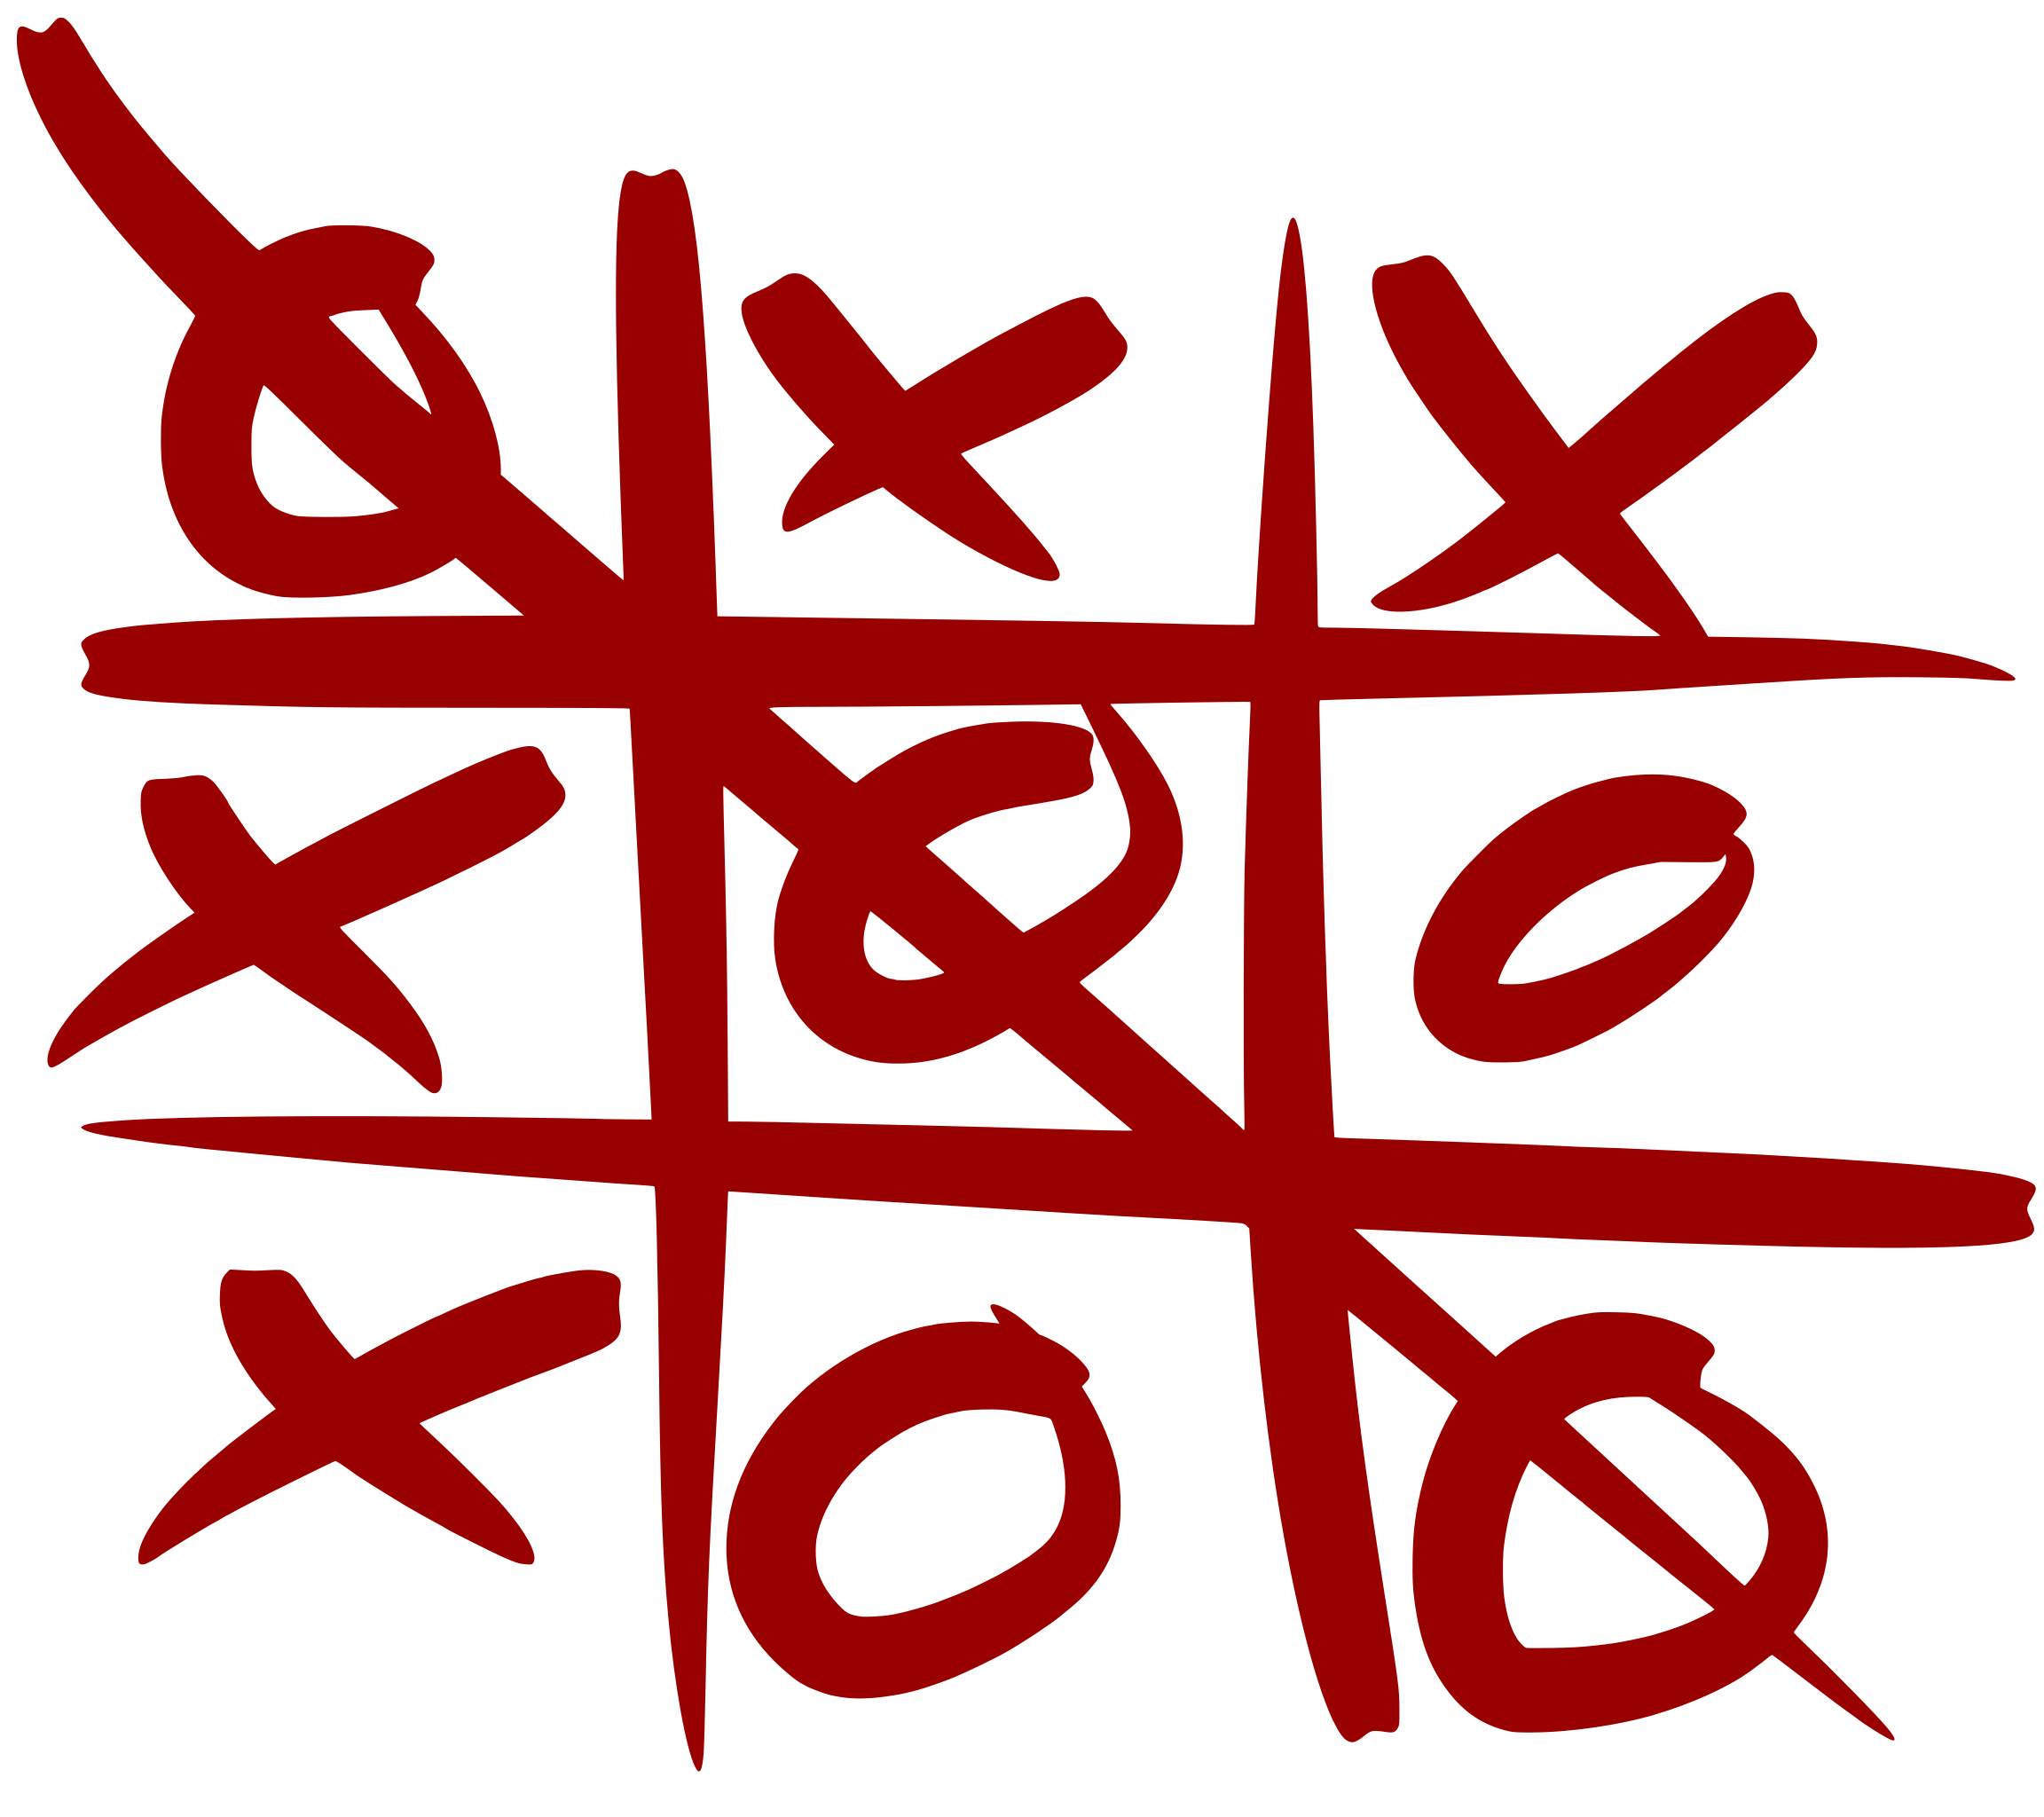
\includegraphics[width=.25\textwidth]{Tic_tac_toe.png} \\
\vspace{\baselineskip}
\scriptsize \url{https://commons.wikimedia.org/wiki/File:Tic_tac_toe.svg}
\caption{The game of Tic-Tac-Toe}
\label{fig:tictactoe}
\end{figure}

Figure~\ref{fig:screen1_chap21} indicates a sequence of moves by the RL agent and the opponent where a starred state (e.g. $c^*$) indicates an optimal state. Beginning from state $a$, the opponent makes the first move and brings the agent to state $b$. The agent then exploits the knowledge about the environment that is reflected in its policy or state value function and chooses the optimal action to move to state $c^*$. The opponent's move leads to state $d$. Now the agent makes an exploratory move and rather than moving to optimal state $e^*$ it moves to state $e$. The opponent moves the state to $f$ and the following action of the agent is exploiting behaviour again. 


\begin{figure}
\centering
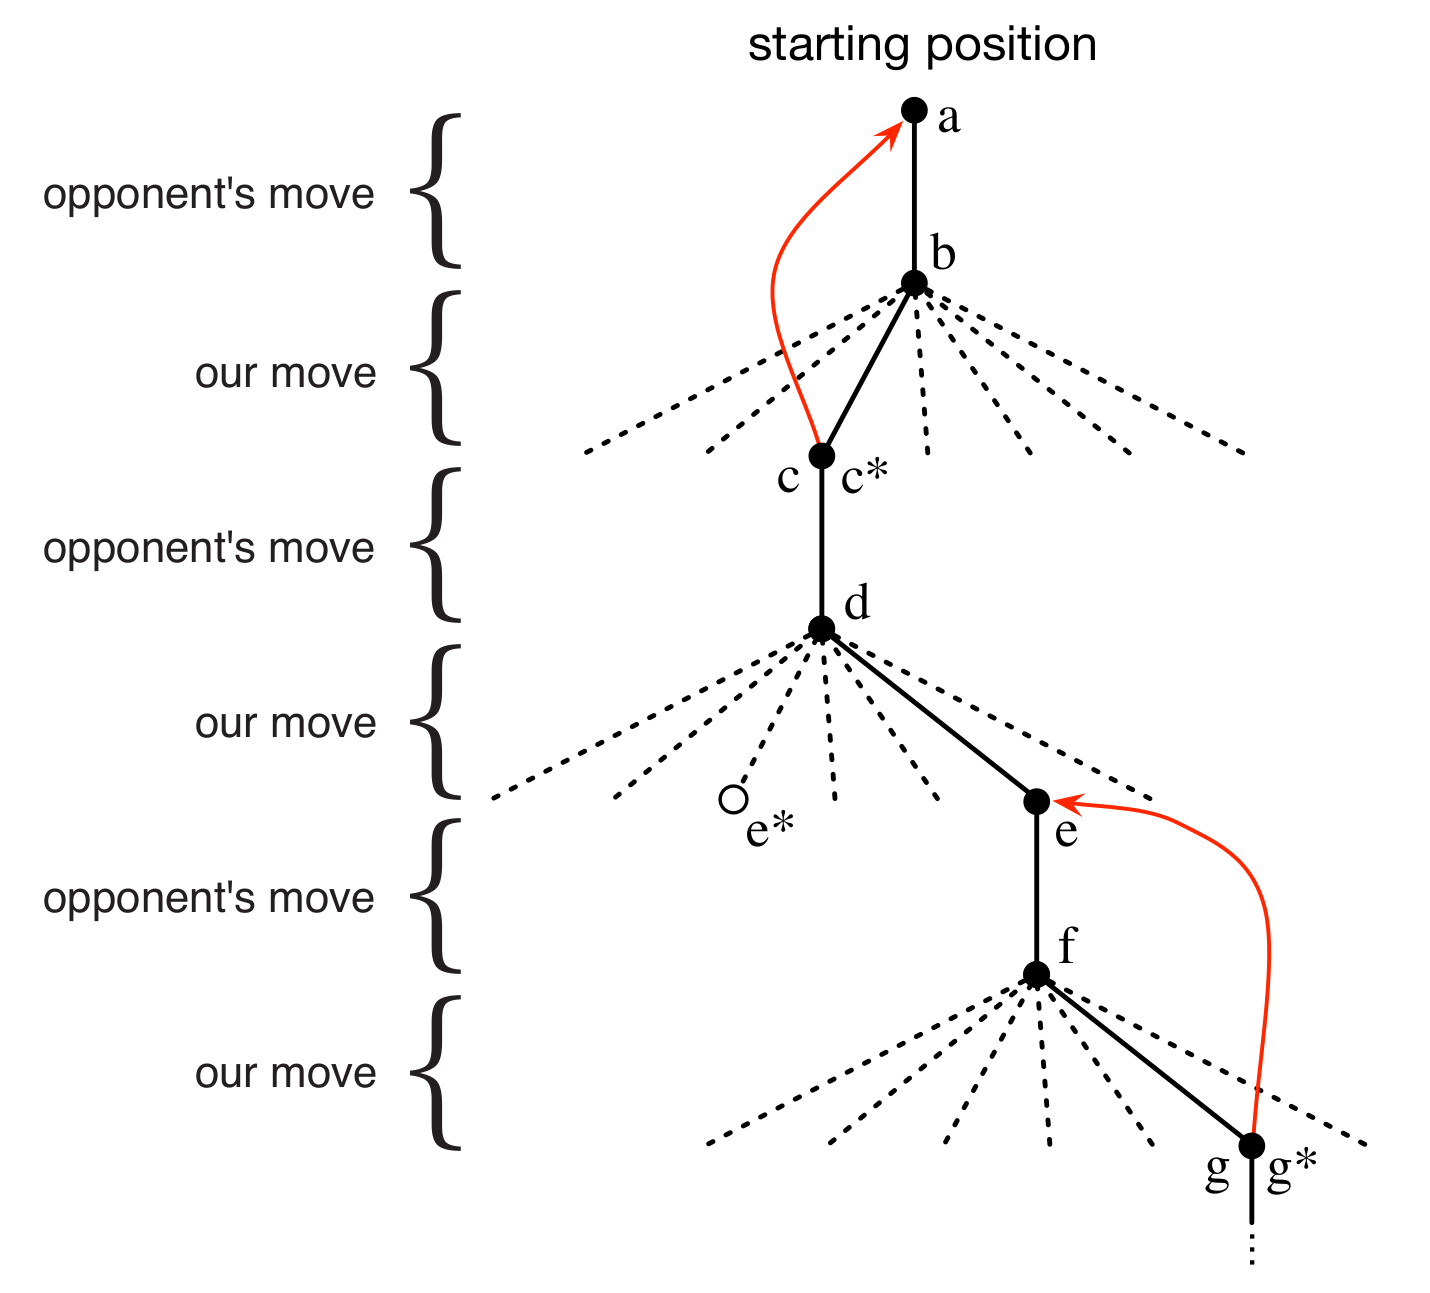
\includegraphics[width=.75\textwidth]{screen1.png} \\
\centering
\scriptsize Source: SB Figure 1.1
\caption{Exploration and exploitation in an RL environment}
\label{fig:screen1_chap21}
\end{figure}

Behaviour that exploits knowledge about the environment, that is, the current action value function and policy, is called \emph{greedy} behaviour as it seeks to maximize the value of the next state. In contrast, exploratory behaviour is typically \emph{random} behaviour. 

After each greedy action from state $s_t$, the RL agent updates its value function for the state $s_t$ based on the value of the new state $s_{t+1}$. The intuition is that if the optimal action from an initial state of low value results in a new state of high value then the value of the initial state should reflect this. In other words, the updated value of the initial state should be closer to that of the final state. This leads to the central \emph{update rule} in \emph{temporal-difference learning}:

\begin{align}
V(S_t) \leftarrow V(S_t) + \alpha \left[ V(S_{t+1}) - V(S_t)\right] \label{eq:1}
\end{align}

Here, $V$ is the value function, and $\alpha$ is a \emph{step size} that determines the rate of update or learning. The term $V(S_{t+1}) - V(S_t)$ is called the \emph{error} and the term $V(S_{t+1})$ is called the \emph{update target}\index{Update target}.

\subsubsection*{Applications in Business and Management}

There are many applications for reinforcement learning in business and management. Consider the following examples:

\begin{itemize}
\item \emph{Dynamic Pricing}: Dynamic pricing involves setting flexible prices for products or services based on current market demands. RL algorithms can help businesses optimize pricing strategies in real-time by learning from consumer behavior and competitor actions, maximizing revenue or market share.

\item \emph{Supply Chain Optimization}: In supply chain management, RL can optimize inventory levels, improve logistics, and manage the supply chain network's dynamic environment. By learning from historical data and ongoing operations, RL algorithms can make adjustments to inventory and shipping strategies, reducing costs and improving service levels.

\item \emph{Customer Interaction Management}: Reinforcement learning can enhance customer relationship management systems by learning to tailor interactions based on customer behavior. This includes optimizing marketing strategies, personalizing recommendations, and improving customer service, all aimed at enhancing customer satisfaction and loyalty.

\item \emph{Financial Portfolio Management}: In finance, RL can be used for portfolio management, where the goal is to optimize the allocation of assets in a portfolio over time. RL algorithms can adapt to changes in market conditions, learning to maximize returns or minimize risk based on the investment strategy.

\item \emph{Manufacturing Process Optimization}: RL algorithms can be applied to control and optimize manufacturing processes by continuously learning and adapting to new data. This can include adjustments to machine settings, production schedules, and maintenance plans to optimize efficiency and reduce operational costs.
\end{itemize}

\section{K-Armed Bandits}

To introduce RL learning, consider the k-armed bandit problem\index{K-armed bandit}. It is named after the nickname of early slot machines (Figure~\ref{fig:bandit}). The RL agent is faced with $k$ such slot machines that give different stochastic rewards. The rewards given by each of the $k$ bandits are initially unknown to the agent. The goal of the agent is to find a policy of which bandit to play in order to maximize the return, that is, the sum of future rewards.

\begin{figure}
\centering

\includegraphics[width=.25\textwidth]{one-armed_bandit.jpg}\\
\tiny \url{https://commons.wikimedia.org/wiki/File:Antique_one-armed_bandit,_Ventnor,_Isle_of_Wight,_UK.jpg}
\caption{An ''one-armed bandit'' slot machine}
\label{fig:bandit}
\end{figure}

The k-armed bandit problem is a very simple RL problem because it is \emph{stateless}. That is, the agent is only ever in one state and the state does not change. This means that the action value function depends only on the action, not the state-action pair.

Formally, there are $k$ possible actions $A_t$ at time $t$ with stochastic reward $R_t$. The action value for each action can be defined as the average reward for that action:

\begin{align*}
   Q_t(a) = \frac{\sum_{i=1}^{t-1} R_i \times \mathbbm{1}_a}{\sum_{i=1}^{t-1} \mathbbm{1}_a} \qquad \text{(average reward)}
\end{align*}

Here $\mathbbm{1}_a$ is 1 when action $a$ has been taken and 0 when another action has been taken. 

A suitable policy that balances exploitation of existing knowledge and exploration for gathering new knowledge is the \emph{$\epsilon$-greedy policy}. An $\epsilon$-greedy policy\index{Policy!Epsilon-greedy} is one that with probability $\epsilon$ takes a random action and with probability $1-\epsilon$ takes the optimal action:

\begin{align*}
A_t = \operatorname*{arg max}_a Q_t(a)
\end{align*}

An incremental implementation of the action value function simply updates the running average when a new reward is received, as follows:

\begin{align}
Q_{t+1}(a) = Q_t(a) + \frac{1}{t}\left[R_t(a) - Q_t(a)\right] \label{eq:2}
\end{align}

Note how the form of Equations~\ref{eq:1} and \ref{eq:2} is similar. They represent different cases of the general \emph{update rule for estimates}:

\begin{align*}
NewEstimate \leftarrow OldEstimate + StepSize \left[ Target - OldEstimate \right]
\end{align*}

Where $\left[ Target - OldEstimate \right]$ is the \emph{error} in the estimate.

\begin{figure}
\begin{tcolorbox}[colback=code]
\begin{align*}
&\text{Initialize, for $a=1$ to $k$:}\\
&\quad Q(a) \leftarrow 0 \\
&\quad N(a) \leftarrow 0 \\
&\text{Loop forever:} \\
&\quad A \leftarrow \begin{cases} \operatorname*{arg max}_a Q(a) &\qquad \text{with probability}\, 1-\epsilon \\
\text{a random action} &\qquad \text{with probability} 
\, \epsilon
\end{cases} \hspace{1in} \\
&\quad R \leftarrow \operatorname{bandit}(A) \\
&\quad N(A) \leftarrow N(A) + 1 \\
&\quad Q(A) \leftarrow Q(A) + \frac{1}{N(A)} \left[ R - Q(A) \right]
\end{align*}
\end{tcolorbox}
\caption{A simple bandit algorithm (Source: SB)}
\label{fig:karmedbandit}
\end{figure}

A complete k-armed bandit algorithm is shown in peusdocode in Figure~\ref{fig:karmedbandit}. The corresponding implementation in Python is straightforward\footnote{Complete implementation is available at \url{https://github.com/jevermann/busi4720-rl/blob/main/bandits.py}}. The following code block defines a class \texttt{k\_bandit\_agent} that represents an agent. Initialization specifies the number of bandits $k$ in the environment, the parameter $\epsilon$ for the $\epsilon$-greedy policy and the initial value of the action value function, which may be 0 as in the pseudocode in Figure~\ref{fig:karmedbandit}. The method \texttt{determine\_action} is simply the $\epsilon$-greedy policy. The \texttt{train} method for each step determines the action to take, then takes that action in the environment and receives a reward. The agent then updates the action value function as in Equation~\ref{eq:2}.

\begin{samepage}
\begin{pythoncode}
class k_bandit_agent:
    def __init__(self, k, epsilon, initial_value):
        self.k = k
        self.epsilon = epsilon
        self.env = k_bandit_env(k)

        self.Q = [initial_value] * self.k
        self.N = [.0] * self.k

    def determine_action(self):
        if random.uniform(0,1) < self.epsilon:
            # explore
            action = random.randint(0, self.k-1)
        else:
            # exploit
            action = self.Q.index(max(self.Q))
        return action

    def train(self, steps):
        rewards = []
        for step in range(steps):
            action = self.determine_action()
            reward = self.env.step(action)
            self.N[action] += 1
            self.Q[action] = (reward-self.Q[action])/self.N[action]
            rewards.append(reward)
        return rewards
\end{pythoncode}
\end{samepage}

A corresponding environment for the agent to act in is also readily implemented in Python and shown in the following code block. The initialization of the environment randomly sets the mean rewards of each of the $k$ bandits. Each time a bandit is played, the \texttt{step()} method randomly determines a reward from a standard normal distribution with the mean of the $k$-th bandit.

\begin{samepage}
\begin{pythoncode}
class k_bandit_env:
    def __init__(self, k):
        self.k = k
        self.mean_rewards = []

        for i in range(self.k):
            self.mean_rewards.append(random.normalvariate(0, 1))

    def step(self, action):
        mean = self.mean_rewards[action]
        reward = random.normalvariate(mean, 1)
        return reward
\end{pythoncode}
\end{samepage}

Figure~\ref{fig:banditresults} shows a comparison of learning behaviour for agents with different parameters $\epsilon$. The horizontal axis shows the index of 1000 steps in the environment and the vertical axis shows the reward received at each step (mean over 1000 runs of the algorithm). The agent with $\epsilon=0$ (blue line) shows the worst learning behaviour. That agent only exploits and never explores. In other words, it never finds any better or more valuable actions to take, once it has found a good action. In contrast, the agent with $\epsilon=0.01$ (red line) learns slower in the beginning as it explores more but after 1000 steps has achieved a better mean reward. Finally, the purple line represents an agent with $\epsilon=0$ but whose action value function has been ''optimistically'' initialized with values of 5 instead of 0, that is, above the expected reward. This prevents it from assuming the first good action is the best one, which leads to high initial learning. However, with an $\epsilon$ of 0, that agent is not capable of further learning later in the sequence of actions taken. 

\begin{figure}
\centering

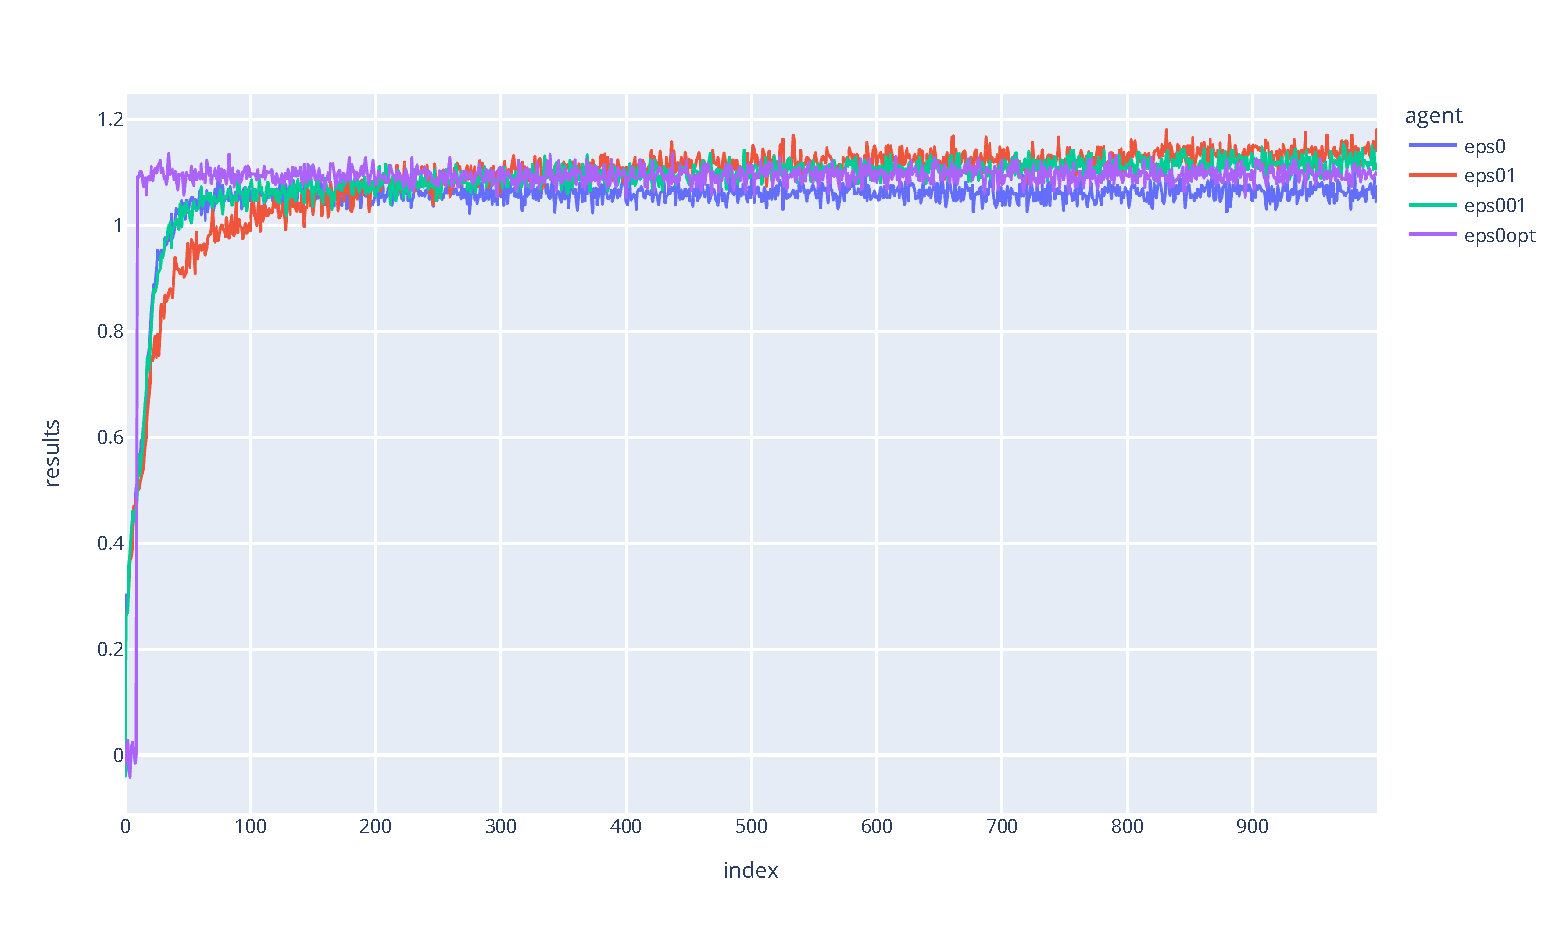
\includegraphics[width=.9\textwidth]{bandits.pdf}
\caption{Learning performance for k-armed bandit agents for different $\epsilon$ and initial action-values}
\label{fig:banditresults}
\end{figure}

\section{Markov Decision Processes and Dynamic Programming}

This section introduces the concept of \emph{Markov decision processes}\index{Markov decision process}, that is, a sequence of decisions or actions and states that has the Markov property: the reward and next state depend only on the current state and action, not on the state history.

\begin{figure}[h]
\centering
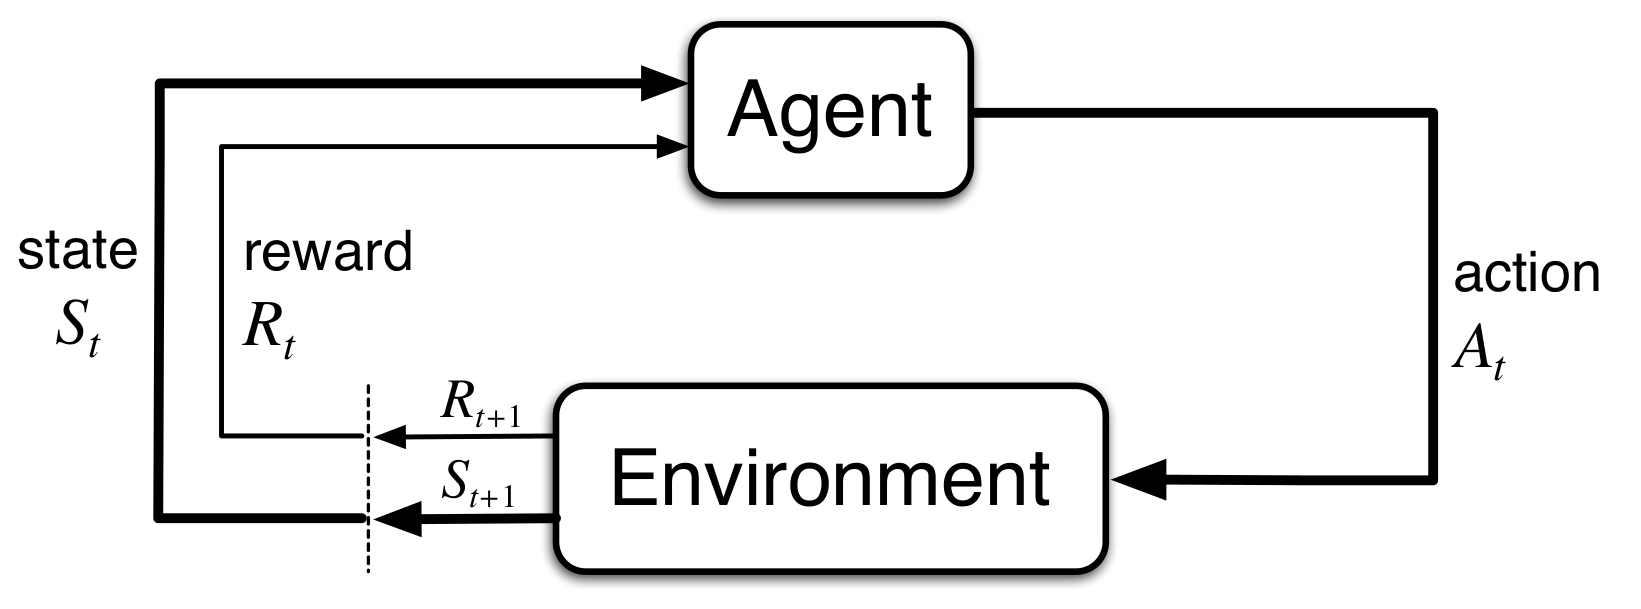
\includegraphics[width=0.75\textwidth]{screen3.png} \\

\scriptsize Source: SB Figure 3.1 \normalsize
\caption{RL agent and environment}
\label{fig:sb31}
\end{figure}

One can think of RL learning as a Markov decision process. Figure~\ref{fig:sb31} shows the RL agent and the environment it is situated in. The environment is at time $t$ in state $S_t$. The agent takes action $A_t$ in the environment and receives reward $R_t$. As a result, the environment's state changes to the new state $S_{t+1}$. This leads to the concept of a \emph{trajectory} as a sequence of states, actions, and rewards:

\begin{align*}S_0, A_0, R_1, S_1, A_1, R_2, \ldots
\end{align*}

\subsection{Definitions}

The behaviour of the environment\index{Environment} is stochastic and can be described through the ''p-function'' which expresses the state transition and reward probabilities. This is known as the \emph{dynamics} of the environment: 
\begin{align}p(s', r | s, a) = \operatorname{Pr}\{S_t = s', R_t =r | S_{t-1} = s, A_{t-1} = a \} \label{eq:dynamics}
\end{align}

The \emph{return}\index{Return (in reinfocement learning)} is formally defined as the possibly discounted sum of future rewards:

\begin{align}
G_t &= R_{t+1} + \gamma R_{t+2} + \gamma^2 R_{t+3} + \cdots = \sum_{k=0}^{\infty} \gamma^k R_{t+k+1} \nonumber \\
    &= R_{t+1} + \gamma G_{t+1} \label{eq:return}
\end{align}

The \emph{state value function}\index{State value function} of state $s$ under a policy $\pi$ is defined as the expected value of the return in that state where $\mathbbm{E}_{\pi}$ is the expection when acting according to policy $\pi$:

\begin{align}
v_\pi(s) &= \mathbbm{E}_\pi [ G_t | S_t = s]  \label{eq:statevalue1} \\
&= \mathbbm{E}_\pi \left[ \sum_{k=0}^\infty \gamma^k R_{t + k + 1} | S_t = s \right] \nonumber
\end{align}

Similarly, the \emph{action value function}\index{Action value function} of state $s$ and action $a$ for policy $\pi$ is defined as the expected return of being in state $s$ and taking action $a$:

\begin{align}
q_\pi(s, a) &= \mathbbm{E}_\pi [ G_t | S_t = s, A_t = a] \label{eq:actionvalue} \\
&= \mathbbm{E}_\pi \left[ \sum_{k=0}^\infty \gamma^k R_{t + k + 1} | S_t = s, A_t = a \right] \nonumber
\end{align}

\subsection{Bellman Equations and Iterative Policy Evaluation}

Starting with Equation~\ref{eq:statevalue1} and substituting Equation~\ref{eq:return} into it yields:

\begin{align}
v_\pi(s) &= \mathbbm{E}_\pi [ G_t | S_t = s] \nonumber \\
&= \mathbbm{E}_\pi [R_{t+1} + \gamma G_{t+1} | S_t = s] \nonumber
\intertext{An expectation is the sum of values weighted by their probability. Summing over all possible combinations of action $a$, next state $s'$ and rewards $r$ and using the dynamics of the environment (Equation~\ref{eq:dynamics}) and the stochastic policy $\pi(a | s)$ for probabilities of taking action $a$ in state $s$, then yields:}
v_\pi(s)  &= \sum_a \sum_{s'} \sum_r \left[ r + \gamma \mathbbm{E}_\pi [ G_{t+1} | S_{t+1} = s'] \right] p(s', r | s, a) \pi(a | s)  \nonumber
\intertext{Note that the expectation of $G_{t+1}$ is not replaced by this sum and remains an expectation. Rearringing this slightly:}
v_\pi(s)  &= \sum_a \pi(a | s) \sum_{s'} \sum_r p(s', r | s, a) \left[ r + \gamma \mathbbm{E}_\pi [ G_{t+1} | S_{t+1} = s'] \right] \nonumber
\intertext{Recognizing that the expectation in the final term on the right is just the state value function (Equation~\ref{eq:statevalue1}) for state $s'$ yields:}
v_\pi(s) &= \sum_a \pi(a | s) \sum_{s', r} p(s', r | s, a) \left[r + \gamma v_\pi(s') \right] \quad \text{for all} \, s \in \mathcal{S} \label{eq:bellman}
\end{align}

Equation~\ref{eq:bellman} is called the \emph{Bellman equation}\index{Bellman equation} for the state value function. A similar equation can be derived for the action value function, beginning with Equation~\ref{eq:actionvalue} and following the same steps. 

To illustrate the concept of the state value function, consider the gridworld example in Figure~\ref{fig:sb32}. An agent is placed on the grid in the left panel of the figure. The agent can take four possible actions; it can move up, down, left or right. Moving off the grid, for example taking action ''up'' when in the top row, results in a reward of $-1$ and the state is unchanged. All other actions yield a reward of $0$ with state changes as indicated by the action, except when states $A$ or $B$ are reached. When reaching state $A$, the agent receives a reward of $+10$ and the next state is $A'$. When reaching state $B$, the agent receives a reward of $+5$ and the next state is $B'$.

The policy $\pi$ in this example is a random policy; independent of its state, the agent takes each action with equal probability. The discount rate is set at $\gamma = 0.9$, favouring immediate rewards over future ones.

The state values for this problem under the random policy are shown in the right panel of Figure~\ref{fig:sb32}. It is clear that being in states $A$ and $B$ is most valuable, as the immediate reward is great. However, the state values are not $+10$ or $+5$ because the agent is likely to incur some negative future rewards. In particular, the state values of the edge states are low or negative because of the probability of falling off the world and incurring a reward of $-1$. 

\begin{figure}
\centering
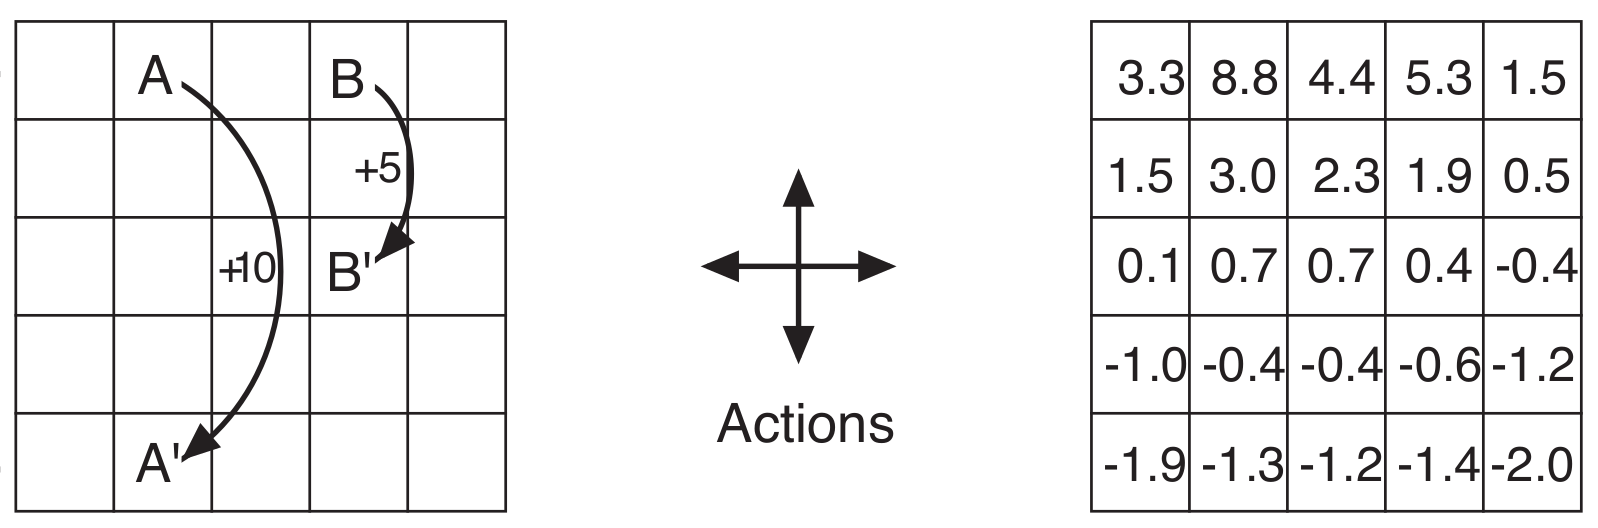
\includegraphics[width=.75\textwidth]{screen4.png} \\

\scriptsize Source: SB Figure 3.2 \normalsize
\caption{Gridworld example and optimal state value function}
\label{fig:sb32}
\end{figure}

The Bellman equation (Equation~\ref{eq:bellman} and its equivalent for the action value function) express the fact that the value of a state (or state-action pair) is a function of the values of all other states (or state-action pairs). This suggests an intuitive way to compute the state values iteratively. Beginning with random values for each state, calculate updated values for all states using Equation~\ref{eq:bellman}. Then, consider the updated values as the current values, and calculate updated values based on these\footnote{In fact, it is not even necessary to wait until all states have been iterated over and updated before using updated state values as current ones.}. Iterate like this until the values do not change any more. It can be proven that this procedure converges to the correct solution and terminates. 


\begin{figure}
\small
\begin{tcolorbox}[colback=code]
\vspace{-\baselineskip}
\begin{align*}
&\text{Loop:} \\
&\quad \Delta \leftarrow 0 \\
&\quad \text{Loop for each}\, s \in \mathcal{S}: \\
&\quad \quad v \leftarrow V(s) \\
&\quad \quad V(s) \leftarrow \sum\nolimits_a \pi(a|s) \sum\nolimits_{s', r} p(s', r|s, a)[r + \gamma V(s')] \hspace{1in} \\
&\quad \quad \Delta \leftarrow \max (\Delta, |v - V(s)|) \\
&\text{until}\, \Delta < \theta
\end{align*}
\end{tcolorbox}
\caption{Iterative Policy Evaluation (Source: SB)}
\label{fig:policyiteration}
\end{figure}

This process is called \emph{iterative policy evaluation}\index{Iterative policy evaluation}. Figure~\ref{fig:policyiteration} shows this in pseudocode and the following Python code block shows the straightforward implementation, beginning with initial values of $0$ for each state.

\begin{samepage}
\begin{pythoncode}
# Define actions for gridworld
A = list(range(0,4))
# Initialize value function V
V = dict()
for state in States:
    V[state] = 0
# Initialize random policy pi
pi = dict()
for state in States:
    pi[state] = random.choice(A)

def evaluate_policy():
    while True:
        Delta = 0
        for s in States:
            v = V[s]
            V[s] = exp_reward(s, pi[s])
            Delta = max(Delta, abs(v - V[s]))
        print(Delta)
        if Delta < theta:
            break
\end{pythoncode}
\end{samepage}


\subsection{Bellman Optimality and Iterative Policy Improvement}

Maximizing the state value function $v$ or action value function $q$ is finding an optimal policy $\pi$, that is, that policy that when following it yields the maximum state value or action value:
\begin{align*}
v_*(s) &= \operatorname*{max}_\pi v_\pi(s) \\
q_*(s, a) &= \operatorname*{max}_\pi q_\pi(s, a)
%\intertext{$q_*$ can be expressed in terms of $v_*$:}
%q_*(s, a) &= \mathbb{E} [ R_{t+1} + \gamma v_* (S_{t+1}) | S_t =s , A_t =a ]
%\end{align*}
\intertext{Intuitively, the value of a state under an optimal policy $\pi_*$ is equal to the expected return for the the best action from that state:}
v_*(s) &= \max_{a \in \mathcal{A}(s)} q_{\pi_*} (s, a)
\intertext{Substituting the definition of the action value function (Equation~\ref{eq:actionvalue}):}
&= \max_a \mathbb{E}_{\pi_*} [ G_t | S_t =s , A_t = a ] 
\intertext{Substituting the recursive definition of the return (Equation~\ref{eq:return}):}
&= \max_a \mathbb{E}_{\pi_*} [R_{t+1} + \gamma G_{t+1} | S_t =s, A_t =a ] 
\intertext{Noting that the expected future return is just the value of the next state, that is, using Equation~\ref{eq:statevalue1}:}
&= \max_a \mathbb{E} [ R_{t+1} + \gamma v_* (S_{t+1}) | S_t =s , A_t =a ] 
\intertext{The expectation is the sum over all following states $s'$ and rewards $r$ weighted by their probabilities. Using the dynamics of the environment (Equation~\ref{eq:dynamics}) that describe the probabilities yields:}
v_*(s) &= \max_a \sum_{s', r} p(s', r | s, a) [ r + \gamma v_* (s')]
\end{align*}
Similarly, the action value under an optimal policy $\pi^*$ can be derived as:
\begin{align}
q_*(s, a) &= \mathbb{E} \left[ R_{t+1} + \gamma \max_{a'} q_*(S_{t+1}, a') | S_t = s, A_t =a \right] \nonumber \\
&= \sum_{s', r} p(s', r | s, a) [ r + \gamma \max_{a'} q_* (s', a') ] \nonumber
\end{align}

These final expressions are known as the \emph{Bellman optimality}\index{Bellman optimality} equations for the state and action value functions.

A simple, intuitive way of finding the optimal policy is to find the optimal state value function. The optimal policy is then to take that action that will yield the best following state. However, changing the policy will change the state value function. This intuitive procedure shows that state value function calculation and policy updates should happen alternatingly, until the policy no longer changes. 

\begin{figure}
\begin{tcolorbox}[colback=code]
\small
\vspace{-\baselineskip}
\begin{align*}
&\text{Loop:} \\
&\quad stable \leftarrow true \\
&\quad \text{For each}\, s \in \mathcal{S}: \\
&\quad \quad old\_action \leftarrow \pi(s) \\
&\quad \quad \pi (s) \leftarrow \operatorname*{argmax}\nolimits_a \sum\nolimits_{s', r} p(s', r|s, a) [r + \gamma V(s')] \hspace{1in} \\
&\quad \quad \text{If}\, old\_action \neq \pi(s) \, \text{then} \, stable \leftarrow false \\
&\quad \text{If}\, stable \; \text{then} \\
&\quad \quad \text{return}\, V \approx v_*\, \text{and} \, \pi \approx \pi_* \\
&\quad \text{else} \\
&\quad \quad \text{go to policy evaluation}
\end{align*}
\end{tcolorbox}
\caption{Iterative Policy Improvement (Source: SB)}
\label{fig:policyimprovement}
\end{figure}

Because the state value computation was already demonstrated using iterative policy evaluation above, the procedure for \emph{iterative policy improvement}\index{Iterative policy improvement} is simple, expressed in Figure~\ref{fig:policyimprovement}. The following Python code block illustrates the straightforward implementation:

\begin{samepage}
\begin{pythoncode}
def improve_policy():
    stable = True
    for s in States:
        old_action = pi[s]
        max_r = -math.inf
        max_a = None
        for action in Actions:
            r = exp_reward(s, action)
            if r > max_r:
                max_r = r
                max_a = action
        pi[s] = max_a
        if old_action != pi[s]:
            stable = False
    return stable
\end{pythoncode}
\end{samepage}

Putting both functions, \texttt{evaluate\_policy()} and \texttt{improve\_policy()}, together in an iteration will yield the optimal policy:

\begin{samepage}
\begin{pythoncode}
stable = False
while not stable:
    evaluate_policy()
    stable = improve_policy()

print("Optimal Policy:")
print(pi)
\end{pythoncode}
\end{samepage}

The procedures of \emph{iterative policy evaluation} and \emph{iterative policy improvement} are an example of the more general approach to optimization called \emph{dynamic programming}.

Consider the example of ''Jack's Car Rental'' (example 4.2 in SB). Jack rents cars at 2 locations. Each location can store 20 cars. The number of daily rental requests and rental returns are Poisson distributed. Jack can move a maximum of 5 cars between the two locations overnight. Each move incurs a reward (cost) of $-2$ and each satisfied rental request receives a reward of $+10$. Jack is looking for the optimal policy that specifies how many cars to move from location 1 to location 2 every night. 

The states in this problem are defined as the number of cars in location 1 and 2, for a total of $20 \times 20 = 400$ possible states and 2 actions, defined in the following Python code block\footnote{Complete implementation available at \url{https://github.com/jevermann/busi4720-rl/blob/main/jacks.py}}:

\begin{samepage}
\begin{pythoncode}
States = []
for cars1 in range(21):
    for cars2 in range(21):
        States.append((cars1, cars2))
        
Actions = range(-5, 5+1)
\end{pythoncode}
\end{samepage}

Figure~\ref{fig:jackscars} shows the policies after each iteration of the iterative policy improvement algorithm in Figure~\ref{fig:policyimprovement}, beginning with the random policy in the top left panel of Figure~\ref{fig:jackscars}. Positive values for the policy indicate cars to move from location 2 to location 1, negative values indicate cars to move from location 1 to location 2. The policy improvement converges to the optimal policy after 4 iterations, with the final state value function shown in the bottom right panel of Figure~\ref{fig:jackscars}.

\begin{figure}
\begin{tabular}{ccc}
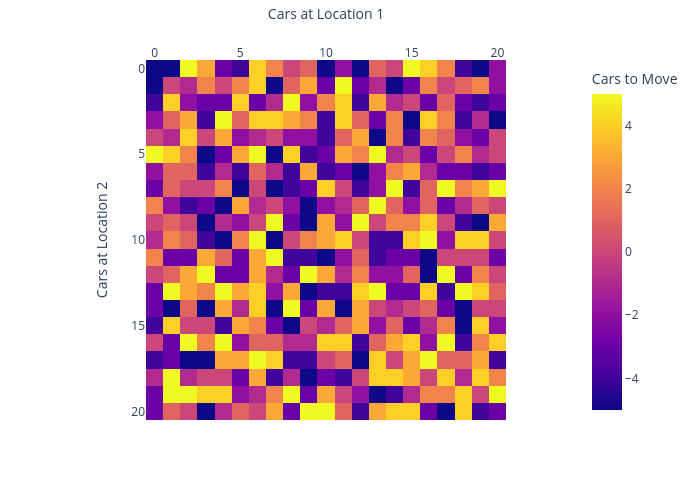
\includegraphics[width=0.3\textwidth]{rl_into/jacks_init_random/jacks_pi_iteration_0.png} &
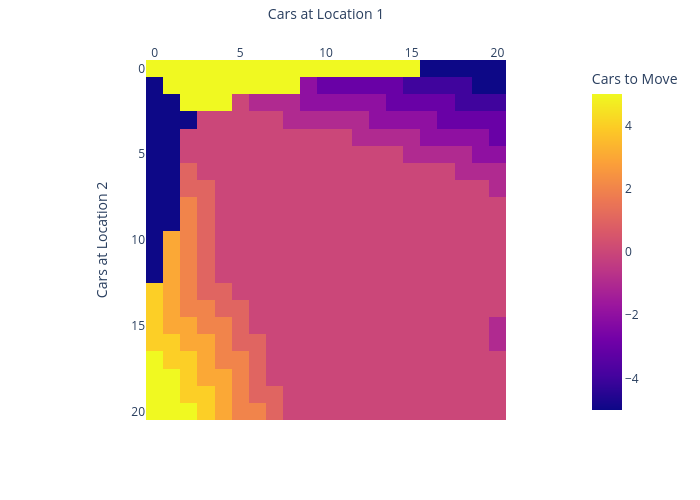
\includegraphics[width=0.3\textwidth]{rl_into/jacks_init_random/jacks_pi_iteration_1.png} &
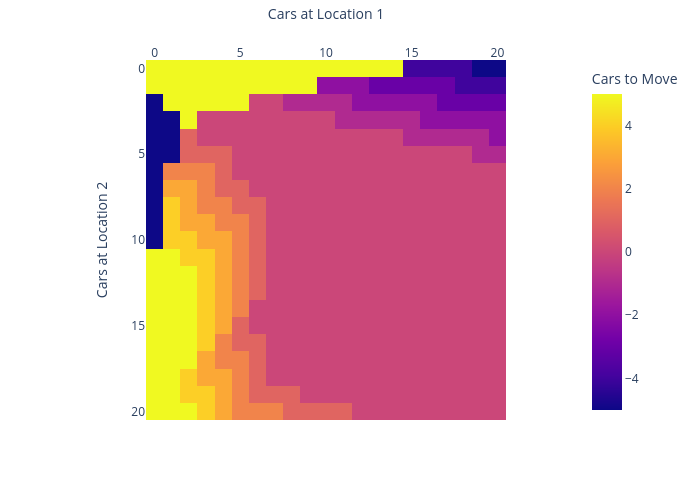
\includegraphics[width=0.3\textwidth]{rl_into/jacks_init_random/jacks_pi_iteration_2.png} \\
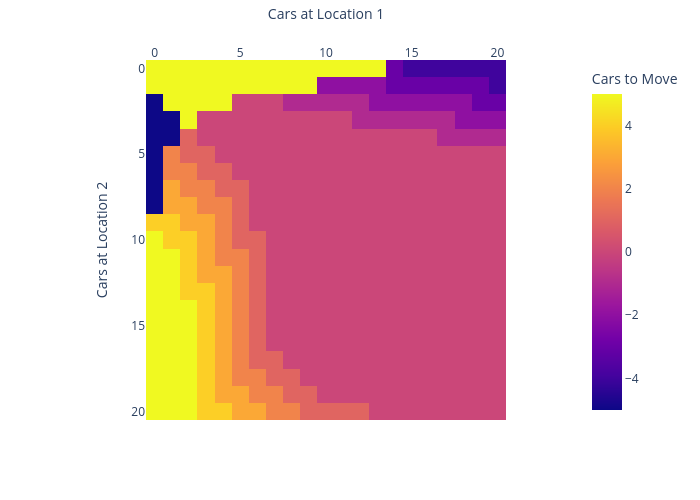
\includegraphics[width=0.3\textwidth]{rl_into/jacks_init_random/jacks_pi_iteration_3.png} &
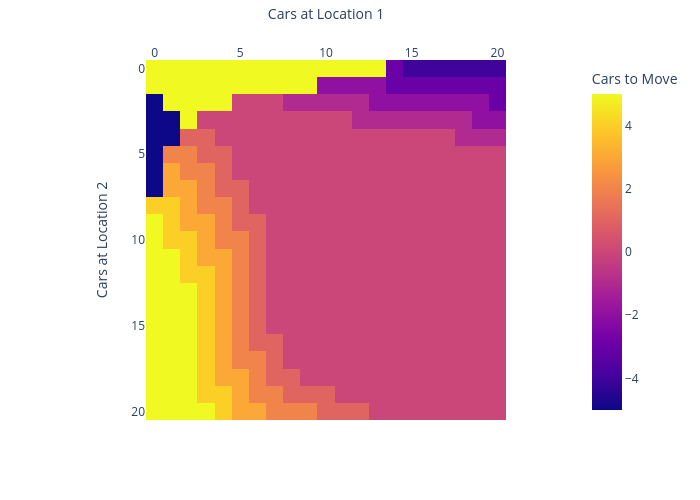
\includegraphics[width=0.3\textwidth]{rl_into/jacks_init_random/jacks_pi_iteration_4.png} &
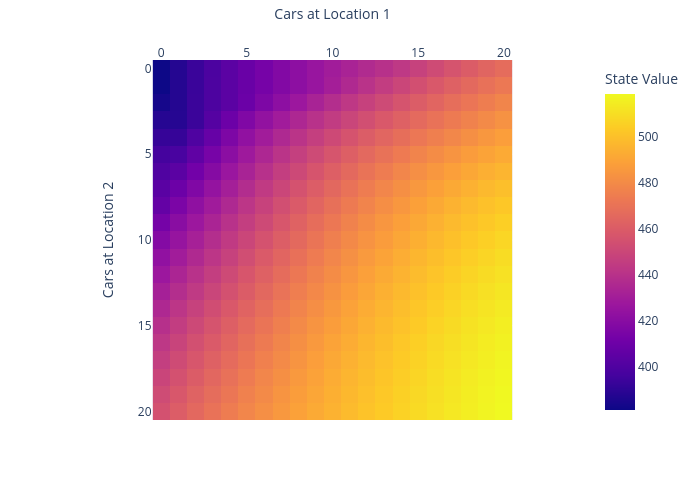
\includegraphics[width=0.3\textwidth]{rl_into/jacks_init_random/jacks_V_iteration_4.png}
\end{tabular}
\caption[Iterative policy improvement example]{Iterative policy improvement example (exercise 4.2 in SB). Policies and final state value function.}
\label{fig:jackscars}
\end{figure}


\section{Monte Carlo (MC) Learning}

The previous section illustrates how optimal policies and their state value and action value function can be computed \emph{under the assumption that the dynamics of the environment, that is Equation~\ref{eq:dynamics}, are known}. In practice, this is not the case --- the $p(s', r | s, a)$ are unknown, there is no model of the environment. The RL agent must learn $V$ and $Q$ from \emph{experience}, that is, it must act in an environment and generate trajectories (sequences of states, actions, and rewards). 

This section assumes \emph{episodic tasks}\index{Episodic task}, that is, problems with a terminal state, a finite trajectory, and finite returns. The agent acts in an environment according to a policy $\pi$ until it arrives in a terminal state and the episode ends. At that point, the entire sequence of states, actions, and rewards is known and state value functions can be estimated or approximated. Recall that the value of a state is the expected return, that is the expected sum of discounted future rewards. State values can then be approximated as the average of the returns in that state. 

A problem arises because the agent can be in the same state multiple times before the episode terminates. Different assumptions can be made. For example, one can assume that it is the first visit of a state that is most influential in determining the outcome of the episode and therefore the state value should be updated with the return at the time of the first visit of a state. Alternatively, one could assume that the last visit of a state is most important, and the value function is updated with the returns at the last time that the state is visited. Yet another alternative is to update the value function for all visits of a state. Figure~\ref{fig:firstvisitmc} shows the pseudocode for this process when the state value function is updated only for the first visit of a state, known as \emph{First-Visit Monte Carlo Prediction}\index{Monte Carlo prediction!first visit}.

\begin{figure}
\begin{tcolorbox}[colback=code]
\small
\vspace{-\baselineskip}
\begin{align*}
& \text{Input: a policy}\;\pi\;\text{ to be evaluated} \\
& \text{Initialize:} \\
& \quad V(s) \in \mathbbm{R}, \text{arbitrarily, for all}\;s \in \mathcal{S} \\
& \quad Returns(s) \leftarrow \text{an empty list, for all}\; s \in \mathcal{S} \\
& \text{Loop forever (for each episode):}\\
& \quad \text{Generate an episode following}\, \pi: S_0, A_0, R_1, S_1, A_1, R_2, \ldots, S_{T-1}, A_{T-1}, R_{T} \\
& \quad G \leftarrow 0 \\
& \quad \text{Loop for each step of episode,}\; t = T-1, T-2, \ldots, 0: \\
& \quad \quad G \leftarrow \gamma G + R_{t+1} \\
& \quad \quad \text{Unless}\; S_t\; \text{appears in}\; S_0, S_1, \ldots, S_{t-1}: \\
& \quad \quad \quad \text{Append}\; G\; \text{to}\; Returns(S_t) \\
& \quad \quad \quad V(S_t) \leftarrow \operatorname{average}(Returns(S_t))
\end{align*}
\end{tcolorbox}
\caption[First-visit MC prediction]{First-visit MC prediction (Source: SB)}
\label{fig:firstvisitmc}
\end{figure}

Note the computation of the return $G$ backwards from the end of the episode. The line ''unless $S_t$ appears in $S_o, S_1, \ldots, S_{t-1}$'' ensures the first-visit property and the final two lines approximate the state value by the average of the returns for that state.

\subsubsection*{Monte Carlo Control}

While Monte Carlo prediction is useful in approximating the state value function, obtaining the optimal policy is done with \emph{Monte Carlo control}\index{Monte Carlo control!first visit}. Instead of approximating $V(S)$ from the returns of an episode, MC control approximates $Q(S, A)$. Figure~\ref{fig:firstvisitcontrol} shows the first-visit MC control algorithm as pseudocode. It is very similar to the first-visit MC prediction algorithm in Figure~\ref{fig:firstvisitmc}. Consider the final three lines: The main change is that returns are assigned not to states, but to pairs of states and actions. The action value function for a state-action pair is approximated as the average over all the returns assigned to it. The optimal policy in some state is that action for wich the action value is maximal. 

There is one additional difference between Figures~\ref{fig:firstvisitmc} and \ref{fig:firstvisitcontrol} in that the initial states and actions of each episode are chosen randomly. This is necessary because the policy $\pi$ in Figure~\ref{fig:firstvisitcontrol} is deterministic and greedy. Without any random influence, there would be no exploration. Forcing episodes to begin with random states and actions is called \emph{exploring starts}\index{Exploring starts} and it ensures that every state-action pair is visited at least once (assuming sufficiently many episodes are generated).

\begin{figure}
\begin{tcolorbox}[colback=code]
\small
\vspace{-\baselineskip}
\begin{align*}
& \text{Initialize for all}\; s \in \mathcal{S}, a \in \mathcal{A} \\
& \quad \pi(s) \in \mathcal{A}(s) \; \text{(arbitrarily)} \\
& \quad Q(s,a) \in \mathbbm{R}\; \text{(arbitrarily)} \\
& \quad Returns(s, a) \leftarrow \text{empty list} \\
& \text{Loop forever (for each episode):} \\
& \quad \text{Choose}\; S_0 \in \mathcal{S}, A_0 \in \mathcal{A}(S_0)\; \text{randomly} \\
& \quad \text{Generate an episode following}\, \pi: S_0, A_0, R_1, S_1, A_1, R_2, \ldots, S_{T-1}, A_{T-1}, R_{T} \\
& \quad G \leftarrow 0 \\
& \quad \text{Loop for each step of episode,}\; t = T-1, T-2, \ldots, 0: \\
& \quad \quad G \leftarrow \gamma G + R_{t+1} \\
& \quad \quad \text{Unless the pair}\; S_t, A_t \; \text{appears in}\; S_0, A_0, S_1, A_1, \ldots, S_{t-1}, A_{t-1}: \\
& \quad \quad \quad \text{Append}\; G\; \text{to}\; Returns(S_t, A_t) \\
& \quad \quad \quad Q(S_t, A_t) \leftarrow \operatorname{average}(Returns(S_t, A_t)) \\
& \quad \quad \quad \pi(S_t) \leftarrow \operatorname*{arg max}_a Q(S_t, a)
\end{align*}
\end{tcolorbox}
\caption[First visit MC control with exploring starts]{First visit MC control with exploring starts (Source: SB)}
\label{fig:firstvisitcontrol}
\end{figure}

As an example of an episodic RL problem that can be usefully learned with MC methods, consider the game of Blackjack (example 5.3 in SB)\footnote{A complete implementation is available at \url{https://github.com/jevermann/busi4720-rl/blob/main/blackjack_es.py}}. In this game,
cards have values A, 2, 3, \ldots, 10 where A is the ace and 10 includes face cards. An ace can count as 1 point or 11 points. An ace that is counted as 11 is called a ''usable ace''. The dealer's initial card is shown. The player can take two possible actions: take another card (''hit'') or do not take a card (''stick''). Once the player sticks, the dealer takes cards. The dealer sticks on a sum of 17 or more. When the player's or the dealer's sum of cards is over 21 they are ''bust'', that is, they lose the game. The dealer's policy is deterministic, they stick on 17 points or more. 

For Blackjack, the states are defined as a combination of the player's current sum of cards, the initial card the dealer is showing, and whether the player has a usable ace (one that can be converted from an 11 to a 1). Actions are to hit or stick. The following Python code block shows how this can be readily implemented:

\begin{samepage}
\begin{pythoncode}
gamma = 1.0
# Define states
States = []
for ace in [0,1]:
    for dealer_showing in range(1,11):
        for hand_sum in range(12, 22):
            States.append((ace,dealer_showing,hand_sum))

# Define actions
Actions = (0, 1)
\end{pythoncode}
\end{samepage}

Initially, the policy is a random policy, action value functions are 0 for all state-action pairs, and the list of returns for each state-action pair is empty:

\begin{samepage}
\begin{pythoncode}
# Initialize policy
pi = dict()
for s in States:
    pi[s] = random.randint(0,1)

# Initialize action value function
Q = dict()
for s in States:
    for a in Actions:
        Q[(s, a)] = 0

# Initialize returns
Returns = dict()
for s in States:
    for a in Actions:
        Returns[(s, a)] = []
\end{pythoncode}
\end{samepage}

The following code block shows the generation of an episode under policy \texttt{pi} from initial state \texttt{s0} and with initial action \texttt{a0}. The function \texttt{step()} calls the environment. It includes the dealer drawing cards after the player uses the ''stick'' action in a state. 

\begin{samepage}
\begin{pythoncode}
def generate_episode(pi, s0, a0):
    terminal = False
    s = s0
    a = a0
    states = [s0]
    actions = [a0]
    rewards = [math.nan]
    while terminal is False:
        sprime, r, terminal = step(s, a)
        rewards.append(r)
        if not terminal:
            aprime = pi[sprime]
            states.append(sprime)
            actions.append(aprime)
            s = sprime
            a = aprime

    return states, actions, rewards, len(rewards)
\end{pythoncode}
\end{samepage}

The core of MC control is implemented in the following Python code block, which is very much analogous to the pseudocode in Figure~\ref{fig:firstvisitcontrol}. Every episode begins in a random state and with a random action. An episode is generated and the sequence of states, actions, returns, and the length of the episode \texttt{T} are returned. Returns are computed from the end of the episode and assigned to the first-visit of a state-action pair. The policy is updated based on the new approximate value of the Q function.

\begin{pythoncode}
# Learn the Q function
for e in range(0, 1000000+1):
    s0 = random.choice(States)
    pi0 = random.choice(Actions)
    S, A, R, T = generate_episode(pi, s0, pi0)
    G = 0
    for t in reversed(range(0, T-1)):
        G = gamma*G + R[t+1]
        if (t == 0) or ((S[t], A[t]) not in zip(S[0:t-1], A[0:t-1])):
            Returns[(S[t], A[t])].append(G)
            Q[(S[t], A[t])] = mean(Returns[(S[t], A[t])])
            if Q[(S[t], 1)] > Q[(S[t], 0)]:
                pi[S[t]] = 1
            else:
                pi[S[t]] = 0
\end{pythoncode}

Figure~\ref{fig:blackjack} shows the resulting policy (left panels) and state value function (right panels) after 1,000,000 learning episodes. The top two plots in Figure~\ref{fig:blackjack} are with a usable ace, the bottom two plots without a usable ace. An action of 1 means to hit, and action 0 is to stand. 

\begin{figure}
\centering

\begin{tabular}{cc}
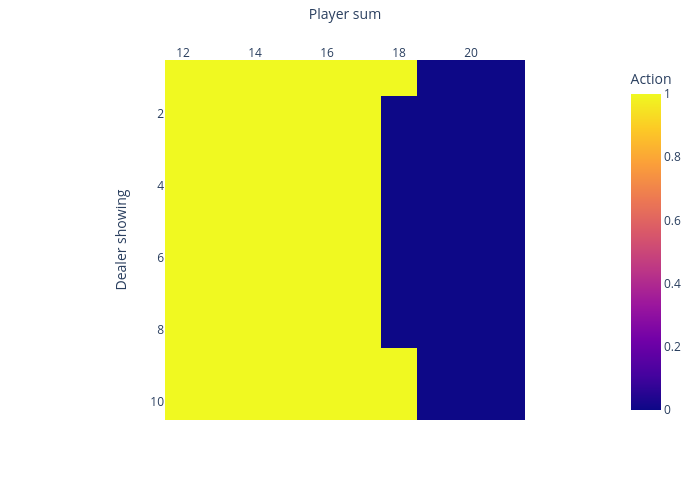
\includegraphics[width=0.4\textwidth]{rl_into/blackjack_es/blackjack_pi_iteration_1000000_ace1.png} &
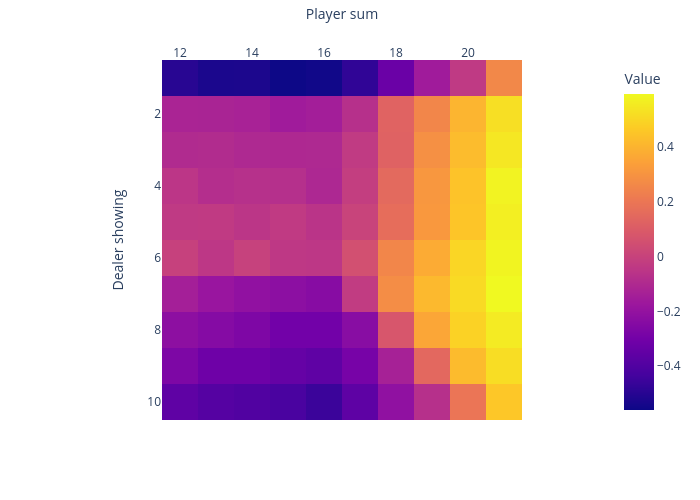
\includegraphics[width=0.4\textwidth]{rl_into/blackjack_es/blackjack_v_iteration_1000000_ace1.png} \\
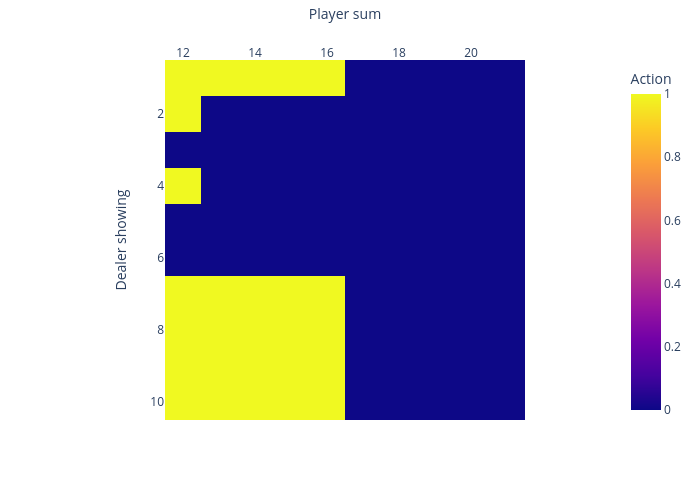
\includegraphics[width=0.4\textwidth]{rl_into/blackjack_es/blackjack_pi_iteration_1000000_ace0.png} &
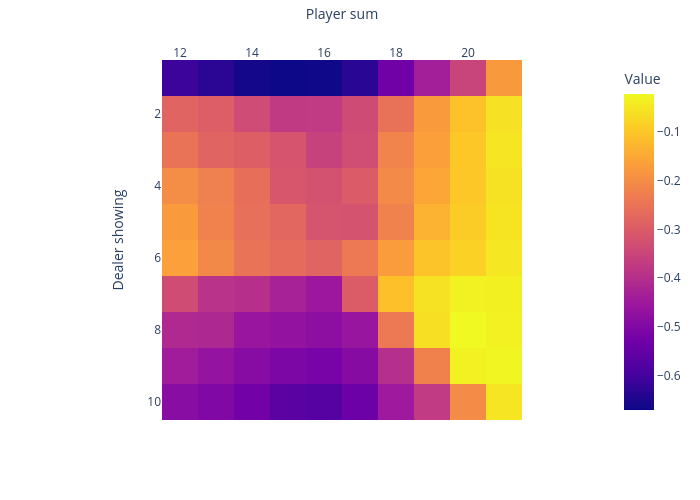
\includegraphics[width=0.4\textwidth]{rl_into/blackjack_es/blackjack_v_iteration_1000000_ace0.png}
\end{tabular}
\caption[Policies and state value function for the Blackjack example]{Policies and state value function for the Blackjack example after 1,000,000 episodes. Usable ace on top, no usable ace at bottom}
\label{fig:blackjack}
\end{figure}

For the game of Blackjack, exploring starts with a deterministic policy is a good way to ensure exploration. However, exploring starts are not always possible or realistic. Instead of using a greedy policy, in those cases an $\epsilon$-soft policy\index{Policy!Epsilon-soft} can be used to ensure exploration. The policy $\pi$ now represents not the action to be taken (greedily, deterministically) but the probability with which each action should be chosen. Consequently, $\pi$ is updated with $\epsilon$-soft probabilities, as shown in the following Python code fragment\footnote{An implementation of the Blackjack problem with an $\epsilon$-soft policy is available at \url{https://github.com/jevermann/busi4720-rl/blob/main/blackjack_eps.py}.}:

\begin{pythoncode}
Q[(S[t], A[t])] = mean(Returns[(S[t], A[t])])
# Optimal policy (for two actions)
A_star = 1 if Q[(S[t], 1)] > Q[(S[t], 0)] else 0

for a in Actions:
    if a == A_star:
        pi[(S[t],a)] = 1-epsilon+epsilon/len(Actions)
    else:
        pi[(S[t],a)] = epsilon/len(Actions)
\end{pythoncode}

An example where exploring starts are not realistic is the Racetrack problem (exercise 5.12 in SB). Cars have to follow the right curve of a racetrack, from the starting line to the finish line, as shown in two examples in Figure~\ref{fig:racetrack}.

\begin{figure}
\centering
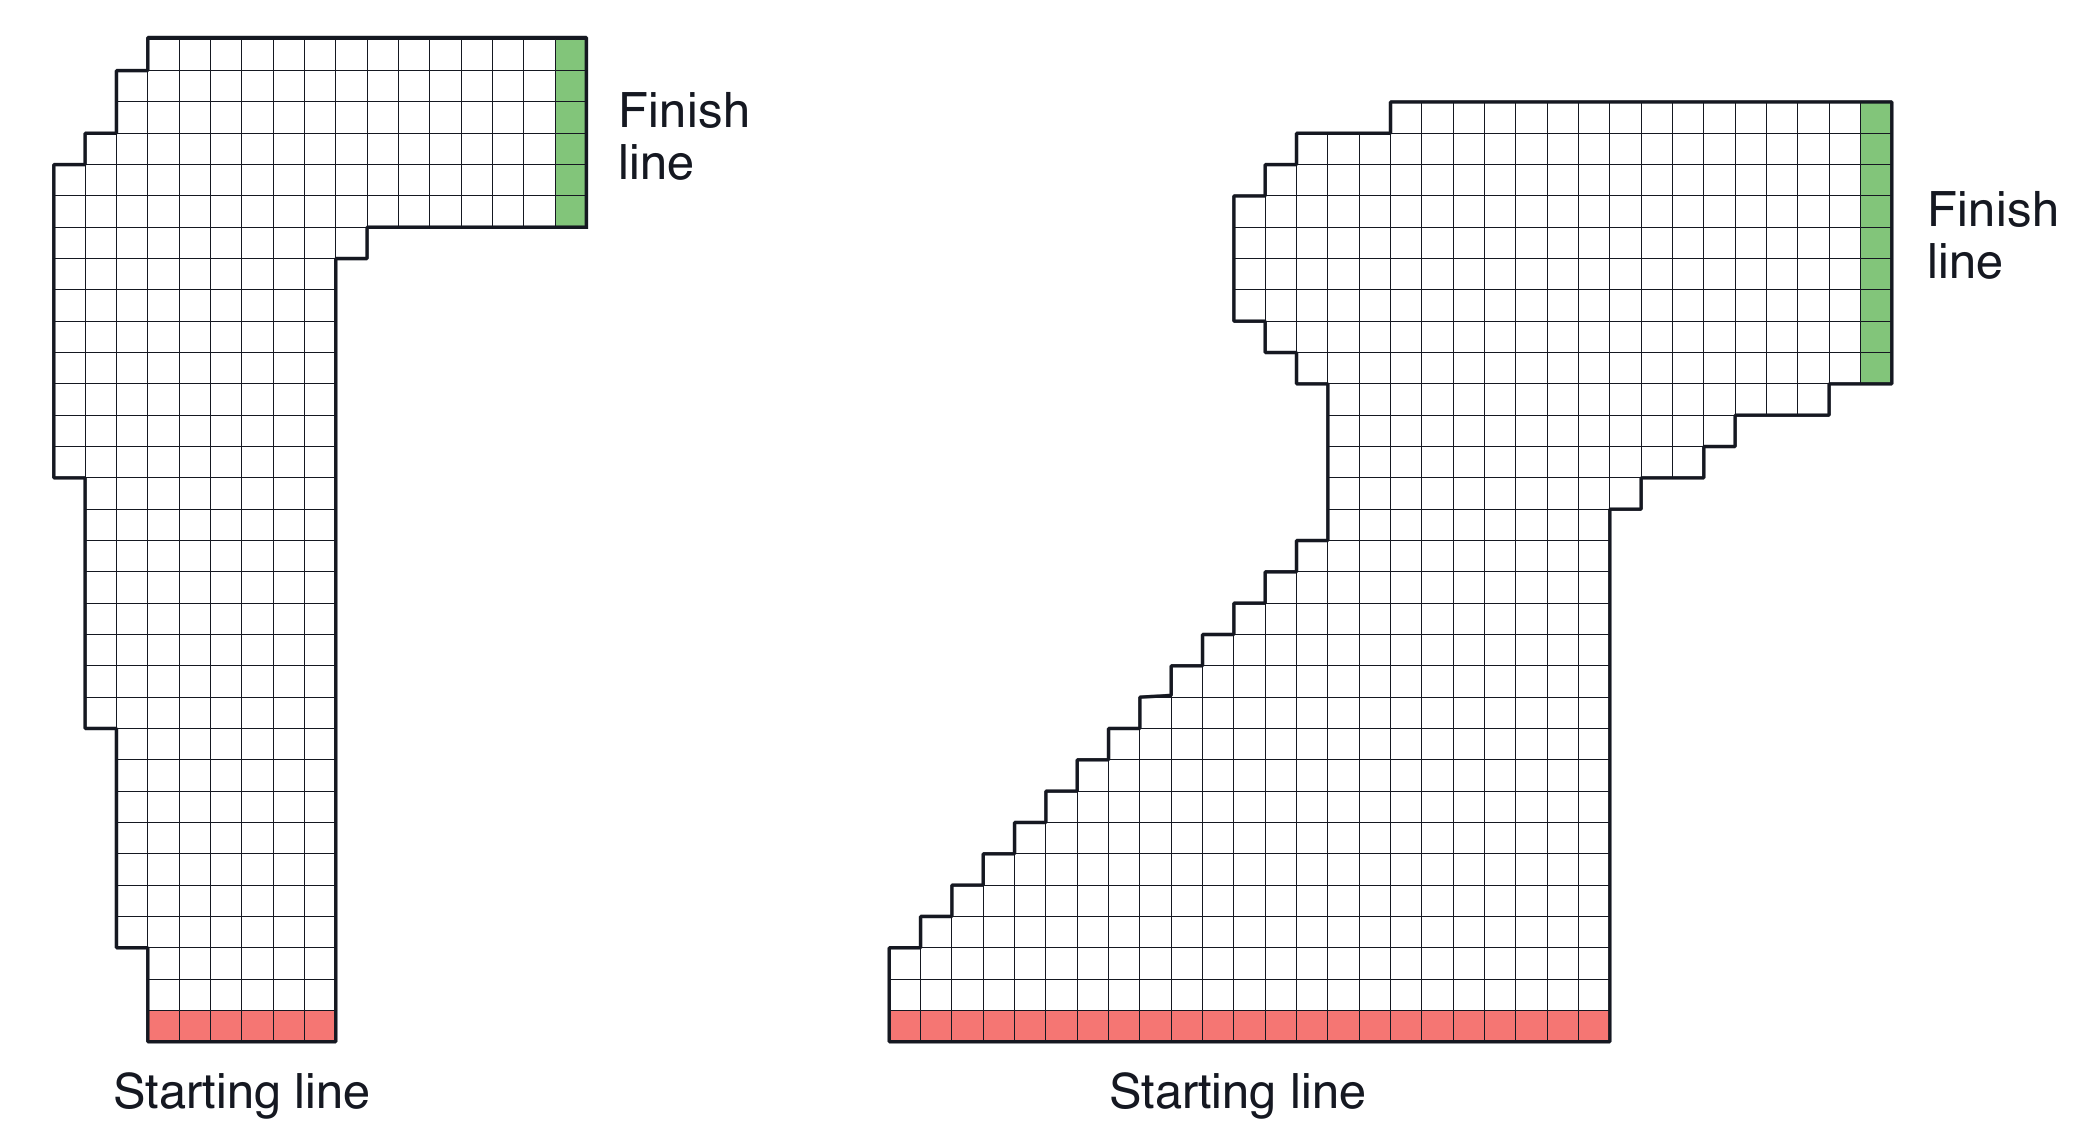
\includegraphics[width=.75\textwidth]{screen5.png} \\
\scriptsize Source: SB Figure 5.5 \normalsize
\caption{Racetrack example}
\label{fig:racetrack}
\end{figure}

The states are defined by the car's position and velocity on the race track, each in two dimensions, horizontally and vertically. The possible actions are to accelerate, coast, or brake in each direction. The rewards are -1 for each step taken and +1 for crossing the finish line, when the episode terminates. When a car moves off the racetrack, it is reset to a random position on the starting line and the episode continues. The environment is stochastic: With a small probability, the actions of the agents are ignored, that is, they have no effect.

The following Python code block defines the actions, the action value function and the $\epsilon$-soft policy that samples from the probability distribution over actions in a state\footnote{Complete implementation is available at \url{https://github.com/jevermann/busi4720-rl/blob/main/racetrack.py}.}
. 

\begin{pythoncode}
Actions = []
for y in range(-1, 2):
    for x in range(-1, 2):
        Actions.append((y,x))

Q = dict()
def getQ(s, a):
    if (s, a) not in Q:
        return 0
    else:
        return Q[(s, a)]

pi = dict()
def get_action(s):
    weights = []
    for a in Actions:
        if (s, a) in pi:
            weights.append(pi[(s, a)])
    return random.choices(Actions, weights=weights)[0]
\end{pythoncode}

The following two Python functions manage the returns for each state-action pair:

\begin{samepage}
\begin{pythoncode}
Returns = dict()
def getReturns(s, a):
    if (s, a) not in Returns:
        return []
    else:
        return Returns[(s, a)]
def appendReturn(s, a, r):
    if (s, a) not in Returns:
        Returns[(s, a)] = [r]
    else:
        Returns[(s, a)].append(r)
\end{pythoncode}
\end{samepage}

The following Python code block represents the core MC control algorithm. Note that the policy \texttt{pi} now represents the probabilities of taking an action in a state and is updated accordingly. The remainder of the code is largely unchanged from the Blackjack example, except that the Racetrack example does not need to use exploring starts, that is, random starting states and actions.

\begin{samepage}
\begin{pythoncode}
for e in range(0, 10000+1):
    S, A, R, T = env.generate_episode()
    G = 0
    for t in reversed(range(0, T-1)):
        G = gamma*G + R[t+1]
        if (t == 0) or ((S[t], A[t]) not in zip(S[0:t-1], A[0:t-1])):
            appendReturn(S[t], A[t], G)
            Q[(S[t],A[t])] = mean(getReturns(S[t],A[t]))
            A_star = argmaxQ(S[t])
            for a in Actions:
                if a == A_star:
                    pi[(S[t],a)]=1-eps+eps/len(Actions)
                else:
                    pi[(S[t],a)]=eps/len(Actions)
\end{pythoncode}
\end{samepage}

Figure~\ref{fig:racetrackresults} shows visualizations of the trajectory of a car (green line) on the racetrack after 0, 100, 200, and 10,000 episodes. It is clear from these trajectories that the number of steps is reduced as training progresses.

\begin{figure}
\centering

\begin{tabular}{cc}
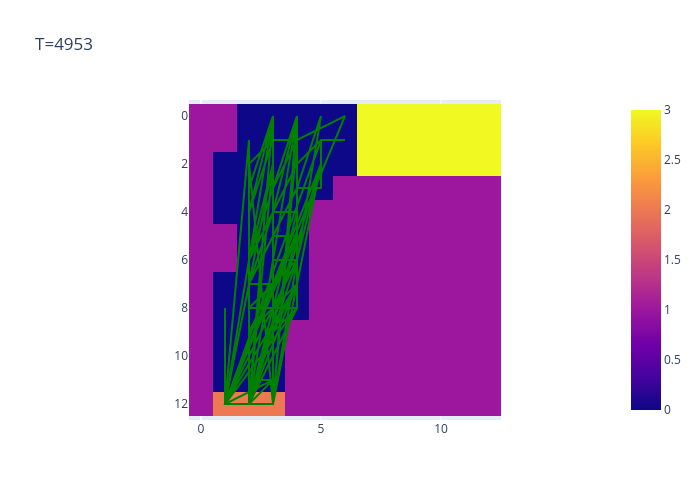
\includegraphics[width=0.45\textwidth]{rl_into/racetrack/racetrack_iteration_0.png} &
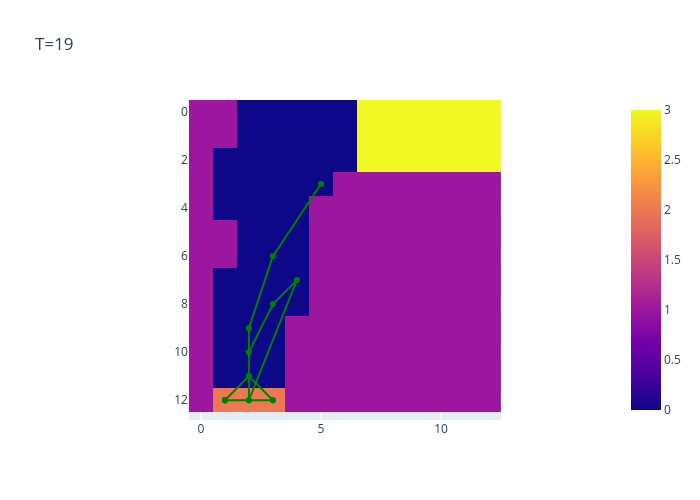
\includegraphics[width=0.45\textwidth]{rl_into/racetrack/racetrack_iteration_100.png} \\
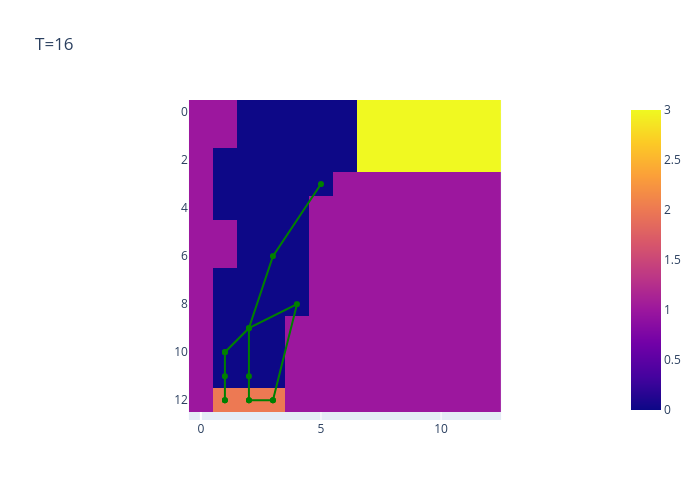
\includegraphics[width=0.45\textwidth]{rl_into/racetrack/racetrack_iteration_200.png} &
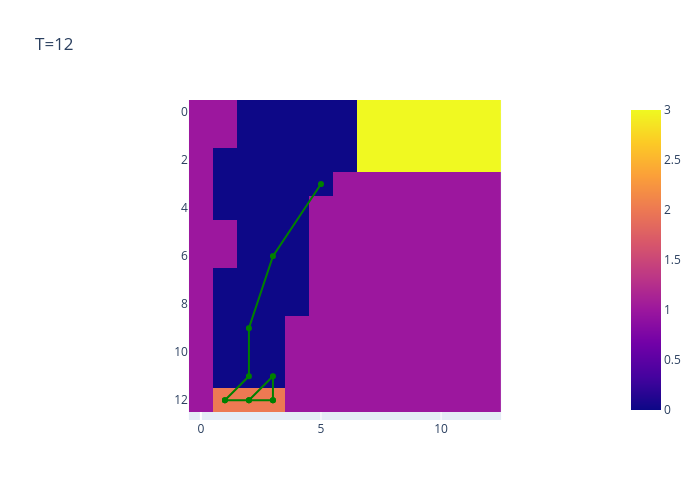
\includegraphics[width=0.45\textwidth]{rl_into/racetrack/racetrack_iteration_10000.png}
\end{tabular}
\caption{Racetrack trajectory after 0, 100, 200, and 10000 learning episodes:
}
\label{fig:racetrackresults}
\end{figure}

\section{Off-Policy MC Learning}

In the MC methods described above, the policy used to generate behaviour (''\emph{behaviour policy}'')\index{Policy!Behaviour}\index{Behaviour policy|see{Policy!Behaviour}}, and the policy that is learned (''\emph{target policy}'')\index{Policy!Target}\index{Target policy|see{Policy!Target}} are the same. However, the need to keep exploring, that is, to behave sub-optimally, when a better, greedy policy could be available, means that the agent's performance is reduced. \emph{Off-policy learning}\index{Off-policy learning} is motivated by the need for efficiency and flexibility in learning optimal policies. The main motivation is the ability to learn about the optimal policy independently of the agent's actions. This is useful in environments where exploring all actions is either potentially damaging or costly.

In on-policy methods, the agent learns from the actions it evaluates and takes, meaning the behaviour policy is the same as the target policy. In contrast, off-policy methods allow the agent to learn a policy different from the one it follows. This is beneficial as it permits the use of historical data from other policies, or data generated from exploratory or less optimal policies, to improve a potentially different and more optimal target policy. 

One important requirement in off-policy learning is that the behaviour policy must \emph{cover}\index{Policy coverage} the target policy. That is, all behaviour possible under the target policy must be (eventually) generated by the behaviour policy. This requirement is intuitive, as the target policy cannot learn about behaviour, that is, the effects of actions in states, that is never encountered in a generated episode.

Figure~\ref{fig:offpolicymc} shows pseudocode for off-policy MC control. In this learning method, the behaviour policy $b$ is typically an $\epsilon$-soft policy, as presented above, that allows exploratory behaviour. The target policy $\pi$ is a deterministic, greedy policy, as can be seen in the third-to-last line of Figure~\ref{fig:offpolicymc}.

\begin{figure}
\small
\begin{tcolorbox}[colback=code]
\vspace{-\baselineskip}
\begin{align*}
& \text{Initialize for all}\; s \in \mathcal{S}, a \in \mathcal{A}(s):\\
& \quad Q(s,a) \in \mathbbm{R}\; \text{(arbitrarily)} \\
& \quad C(s, a) \leftarrow 0 \\
& \quad \pi(s) \leftarrow \operatorname{arg max}_a Q(s, a) \\
& \text{Loop forever (for each episode):} \\
& \quad \text{Generate an episode following}\, b: S_0, A_0, R_1, S_1, A_1, R_2, \ldots, S_{T-1}, A_{T-1}, R_{T} \\
& \quad G \leftarrow 0; W \leftarrow 1 \\
& \quad \text{Loop for each step of episode,}\; t = T-1, T-2, \ldots, 0: \\
& \quad \quad G \leftarrow \gamma G + R_{t+1} \\
& \quad \quad C(S_t, A_t) \leftarrow C(S_t, A_t) + W \\
& \quad \quad Q(S_t, A_t) \leftarrow Q(S_t, A_t) + \frac{W}{C(S_t, A_t)} \left[ G - Q(S_t, A_t) \right] \\
& \quad \quad \pi(S_t) \leftarrow \operatorname*{arg max}_a Q(S_t, a) \\
& \quad \quad \text{If}\; A_t \neq \pi(S_t) \; \text{then proceed to next episode} \\
& \quad \quad W \leftarrow W / b(A_t | S_t)
\end{align*}
\end{tcolorbox}
\caption[Off-Policy MC Control]{Off-Policy MC Control (Source: SB)}
\label{fig:offpolicymc}
\end{figure}

The following Python code blocks show how off-policy MC control can be implemented. The first block defines the two policies, the $\epsilon$-soft behaviour policy \texttt{b} and the greedy deterministic policy \texttt{pi}.

\begin{samepage}
\begin{pythoncode}
def b(s):
    weights = []
    for a in Actions:
        if (s, a) in Q:
            weights.append(math.exp(Q[(s, a)]))
        else:
            weights.append(0)
    if len(weights) == 0 or sum(weights) == 0:
        return random.choice(Actions)
    else:
        return random.choices(Actions, weights)[0]

def pi(s):
    a = argmaxQ(s)
    if a is None:
        return random.choice(Actions)
    else:
        return a
\end{pythoncode}
\end{samepage}

Note that the last line of Figure~\ref{fig:offpolicymc} makes reference to the probabilities of action $A_t$ in state $S_t$ under the behaviour policy $b$. This probability is computed by the following Python code block:

\begin{samepage}
\begin{pythoncode}
def bprob(a, s):
    if (s, a) not in Q:
        return 1
    weights = []
    for aa in Actions:
        if (s, aa) in Q:
            weights.append(math.exp(Q[(s, aa)]))
    if len(weights) == 0 or sum(weights) == 0:
        return 1
    else:
        return math.exp(Q[(s, a)]) / sum(weights)
\end{pythoncode}
\end{samepage}

With these definitions, the learning algorithm is a straightforward implementation of the pseudocode in Figure~\ref{fig:offpolicymc}\footnote{Complete implementation using the Racetrack example is available at \url{https://github.com/jevermann/busi4720-rl/blob/main/racetrack_off_policy.py}.}:

\begin{samepage}
\begin{pythoncode}
for e in range(0, 10000+1):
    S, A, R, T = env.generate_episode_b()
    G = 0
    W = 1
    for t in reversed(range(0, T-1)):
        G = gamma*G + R[t+1]
        C[(S[t], A[t])] = getC(S[t], A[t]) + W
        Q[(S[t], A[t])] = getQ(S[t], A[t]) + \
               W/getC(S[t], A[t]) * (G-getQ(S[t],A[t]))
        if A[t] != pi(S[t]):
            break
        else:
            W = W * 1/bprob(A[t], S[t])
\end{pythoncode}
\end{samepage}

\section{Temporal-Difference (TD) Learning}

Temporal Difference (TD) learning\index{Temporal difference learning}\index{TD learning|see{Temporal difference learning}} is an RL approach that combines ideas from both Monte Carlo (MC) methods and dynamic programming. The primary motivation for temporal difference learning stems from its ability to learn predictions based on other learned predictions, a concept referred to as bootstrapping. Unlike Monte Carlo methods, which wait until the completion of an episode to update the value estimates based on actual returns, TD learning updates estimates based on estimate returns, thus not requiring the episode to terminate before updates can be made. This allows TD learning to make more frequent updates, which can accelerate learning, and to be applied in continuing (non-episodic) environments.

Recall that in MC control, the updates to the action value function use the actual return $G_t$ at time $t$ as the target, which can only be computed at the end of an episode:

\begin{align}
Q(S_t, a) &\leftarrow Q(S_t, a) + \alpha \left[ G_t - Q(S_t, a) \right] \nonumber
\intertext{Substituting the recursive definition of the return (Equation~\ref{eq:return}) yields:}
Q(S_t, a) &\leftarrow Q(S_t, a) + \alpha \left[ R_{t+1} + \gamma G_{t+1} - Q(S_t, a) \right] \nonumber
\intertext{Recognizing that the expected value of $G_{t+1}$ is approximated by the $Q$ value of the optimal action in the next state (Equation~\ref{eq:actionvalue}) yields the TD update:}
Q(S_t, a) &\leftarrow Q(S_t, a) + \alpha \left[ R_{t+1} + \gamma Q(S_{t+1}, a_{t+1}^*) - Q(S_t, a) \right] \label{eq:sarsaupdate}
\end{align}

In other words, there is no need to wait until the actual return $G_t$ is known at the end of an episode, as TD learning uses the current approximation or estimate of $G_t$ as the update target. This idea of using estimates to update or compute better estimates is called \emph{bootstrapping}\index{Bootstrapping}. 

Figure~\ref{fig:sarsa} shows the pseudocode of a method called ''\emph{SARSA}''\index{SARSA}, so-called because it uses information of the current state $S$, current action $A$, reward $R$, next state $S'$ and next action $A'$ in its update. SARSA uses the update function defined in Equation~\ref{eq:sarsaupdate}. SARSA is an on-policy method, typically using an $\epsilon$-greedy policy based on $Q$ to generate behaviour and ensure exploration.

\begin{figure}
\small
\begin{tcolorbox}[colback=code]
\vspace{-\baselineskip}
\begin{align*}
& \text{Initialize}\; Q(s, a) \; \text{for all} \; s \in \mathcal{S}^+ \; \text{, arbitrarily} \\
& \text{Loop for each episode:} \\
& \quad \text{Initialize}\; S \\
& \quad \text{Choose} \, A \, \text{from}\, S \, \text{using policy derived from} \, Q \\
& \quad \text{Loop for each step of episode:} \\
& \quad \quad \text{Take action}\, A, \, \text{observe} \, R, S' \\
& \quad \quad \text{Choose}\, A' \, \text{from}\, S' \, \text{using policy derived from} \, Q \\ 
& \quad \quad Q(S, A) \leftarrow Q(S, A) + \alpha \left[ R + \gamma Q(S', A') - Q(S, A) \right] \\
& \quad \quad S \leftarrow S'; A \leftarrow A' \\
& \quad \text{until}\, S\, \text{is terminal}
\end{align*}
\end{tcolorbox}
\caption[TD-control with SARSA]{TD-control with the SARSA method (Source: SB)}
\label{fig:sarsa}
\end{figure}

To illustrate the use of SARSA, consider the ''Windyworld'' example environment (example 6.5 in SB), shown in Figure~\ref{fig:windyworld}. An agent has to move from start state $S$ to terminal goal state $G$ in this gridworld. However, there is a wind on some columns of the grid that pushes the agent towards the top (indicated below the columns in Figure~\ref{fig:windyworld}). Rewards are $-1$ for every step until termination, so that the agent is encouraged to find the path requiring the least number of actions. There are no penalties for moving off the world (the action is simply ignored) and the problem is not discounted ($\gamma=1$).


\begin{figure}
\centering
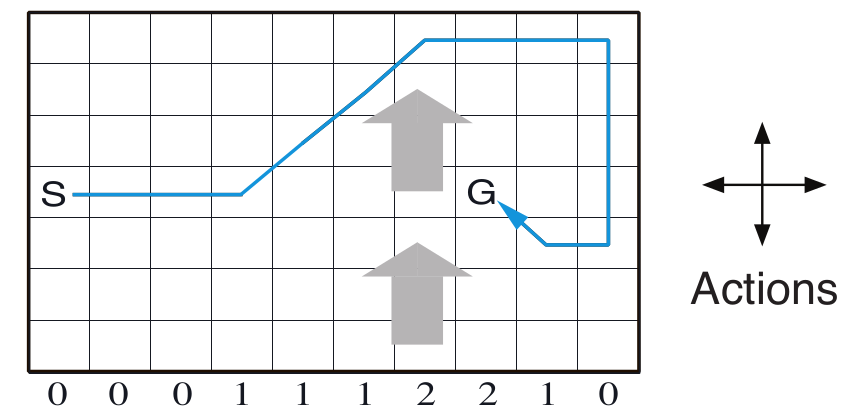
\includegraphics[width=.5\textwidth]{screen6} \\
\scriptsize Source: SB Chapter 6 \normalsize 
\caption{Windyworld example}
\label{fig:windyworld}
\end{figure}

The following python code blocks define the states, actions, and an $\epsilon$-greedy policy \texttt{pi}:

\begin{samepage}
\begin{pythoncode}
# Define states
States = []
for i in range(nrow):
    for j in range(ncol):
        States.append((i, j))

# Define actions
Actions = range(0, 4)
# Initialize Q
Q = dict()
for s in States:
    for a in Actions:
        Q[(s, a)] = random.random()

# Define pi
def pi(s):
    if random.random() < epsilon:
        return random.choice(Actions)
    else:
        return argmaxQ(s)
\end{pythoncode}
\end{samepage}

With these definitions, the implementation of SARSA is straightforward from the pseudocode in Figure~\ref{fig:sarsa}\footnote{A complete implementation of the Windyworld example is available at \url{https://github.com/jevermann/busi4720-rl/blob/main/windyworld_sarsa.py}.} and shown in the following Python code block.

\begin{samepage}
\begin{pythoncode}
for e in range(0, 100):
    terminal = False
    S = windy.reset()
    A = pi(S)
    step = 0
    while terminal is False:
        Sprime, R, terminal = windy.step(A)
        Aprime = pi(Sprime)
        Q[(S,A)] = Q[(S,A)] + alpha*(R + \
            gamma * Q[(Sprime, Aprime)] - Q[(S, A)])
        S = Sprime
        A = Aprime
\end{pythoncode}
\end{samepage}

In summary, Temporal Difference learning and Monte Carlo methods differ primarily in when and how the updates to value estimates are made:
\begin{itemize}
\item \emph{Update Timing:} TD learning updates values at every time step using current estimates, which means it can start learning from incomplete sequences, making it suitable for non-episodic environments. Monte Carlo methods update only at the end of each episode, using the total accumulated return from the episode.
\item \emph{Sampling vs. Bootstrapping:} Monte Carlo methods rely solely on actual returns (full sampling), and do not bootstrap. In contrast, TD methods bootstrap, using existing value estimates to update new estimates.
\item \emph{Convergence Properties:} Due to its incremental nature and frequent updates, TD learning can converge faster in practical applications than Monte Carlo methods, which require longer trajectories and may suffer from higher variance in their estimates due to the complete reliance on actual returns.
\end{itemize}

\subsubsection*{Generalizing TD Learning to N Steps}

In developing the SARSA method (Equation~\ref{eq:sarsaupdate}), the recursive definition of the return (Equation~\ref{eq:return}) and the definition of the action value as the expected return (Equation~\ref{eq:actionvalue}) were applied once. Hence the SARSA update target $R_{t+1} + Q(S_{t+1}, a_{t+1})$ ''looks ahead'' by one step to the next reward $R_{t=1}$ and then approximates the remaining portion of $G_{t+1}$ by $Q(S_{t+1}, a_{t+1})$. This is therefore called the ''1-step'' target, and the update error $\delta$ is called the ''1-step error'':

\begin{align*}
\delta_{TD1} = R_{t+1} + Q(S_{t+1}, a_{t+1}) - Q(S_t, a)
\end{align*}

This can be extended by applying Equations~\ref{eq:return} and \ref{eq:actionvalue} a second time. This yields the ''2-step error'' that looks ahead at the next two rewards, and then approximates the remainder by $Q(S_{t+2}, a_{t+2})$:

\begin{align*}
\delta_{TD2} = R_{t+1} + \gamma R_{t+2} + \gamma^2 Q(S_{t+2}, a_{t+2}) - Q(S_t, a)
\end{align*}

Calculating the 2-step error requires knowledge of two actual rewards, so the 2-step update can be performed only after two steps. Or, viewed from a different perspective, the 2-step update updates not only the value of the most recent state-action pair but the values of the two most recent state-action pairs. 

This can be generalized by applying Equations~\ref{eq:return} and \ref{eq:actionvalue} n-times, yielding the \emph''{n-Step TD error}'':

\begin{align*}
\delta_{TDn} = R_{t+1} + \gamma R_{t+2} + \cdots + \gamma^{n-1} R_{t+n} + \gamma^n Q(S_{t+n}, a_{t+1}) - Q(S_t, a)
\end{align*}

The n-step update can only be performend after $n$ steps have passed so that $n$ actual rewards are available, with the remainder of $G_{t+1}$ being approximated. As an alternative interpretation, the n-step update changes the values of the last $n$ state-action pairs in the trajectory. Figure~\ref{fig:sarsa10step} shows an illustration of this for 10-step SARSA\index{n-step TD learning}.


\begin{figure}
\centering
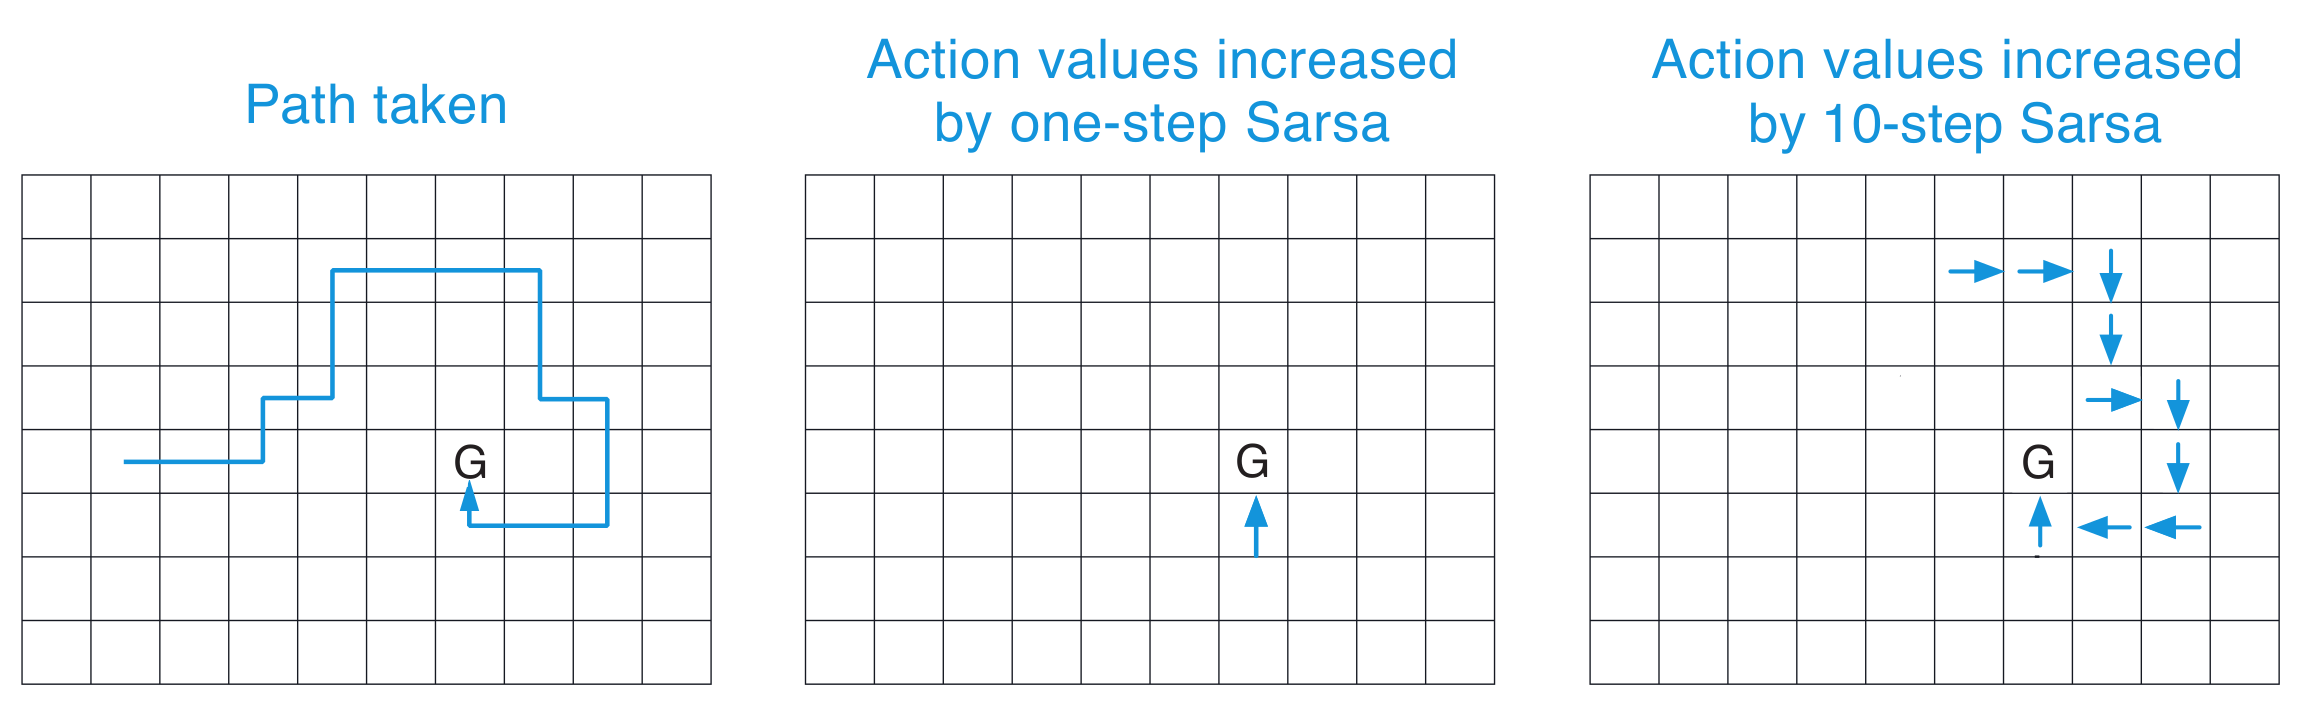
\includegraphics[width=\textwidth]{screen7.png}

\scriptsize
Source: SB Figure 7.4
\caption{SARSA versus n-Step TD Learning (n-step SARSA)}
\label{fig:sarsa10step}
\end{figure}


\section{Off-Policy TD Learning}

Temporal Difference learning can be combined with off-policy learning as well. A popular method for this is Q-learning\index{Q-learning}. Q-learning updates the action values in a greedy way, that is, of a greedy policy, regardless of the action taken by the policy being followed (the behavior policy). The differences between SARSA and Q-learning are minor. Importantly, it is not necessary to explicitly encode the behaviour and target policies.

Consider the following aspects of SARSA. The next action $A'$ that is carried out is determined using a (behaviour) policy based on $Q$ and $Q$ is being learned (updated) based on the actually taken action $A'$ (target policy). This makes SARSA an on-policy method.

\begin{tcolorbox}[colback=code]
\setlength{\abovedisplayskip}{0pt}
\setlength{\belowdisplayskip}{0pt}
\setlength{\abovedisplayshortskip}{0pt}
\setlength{\belowdisplayshortskip}{0pt}
\subsubsection*{SARSA (on-policy):} 

\begin{align*}
& \text{Take action}\, A, \, \text{observe} \, R, S' \\
& \text{Choose}\, A' \, \text{from}\, S' \, \text{using policy derived from} \, Q \\ 
&  Q(S, A) \leftarrow Q(S, A) + \alpha \left[ R + \gamma Q(S', A') - Q(S, A) \right] \hspace{1in}\\
&  S \leftarrow S'; A \leftarrow A'
\end{align*}
\end{tcolorbox}

A minor change is sufficient to change on-policy SARSA to off-policy Q-learning, shown in the box below. Here, the next action $A$ that is carried out is also determined using a (behaviour) policy based on $Q$, but $Q$ is updated not based on the actually taken action $A$, but based on the optimal action $A'$, that is, the action with the maximum $Q$ value in the following state $S'$. This difference means that the policy that governs behaviour (''behaviour policy'') is different than the policy that is updated or learned (''target policy''), making Q-learning an off-policy method. 

\begin{tcolorbox}[colback=code]
\setlength{\abovedisplayskip}{0pt}
\setlength{\belowdisplayskip}{0pt}
\setlength{\abovedisplayshortskip}{0pt}
\setlength{\belowdisplayshortskip}{0pt}
\subsubsection*{Q-learning (off-policy):}

\begin{align*}
& \text{Choose} \, A \; \text{from}\, S \; \text{using policy derived from} \, Q \\
& \text{Take action}\, A, \, \text{observe} \, R, S' \\
&  Q(S, A) \leftarrow Q(S, A) + \alpha \left[ R + \gamma \operatorname*{max}_a Q(S', A') - Q(S, A) \right] \hspace{.6in}\\
& S \leftarrow S'
\end{align*}
\end{tcolorbox}

The corresponding Python implementation for the Windyworld example is also straightforward from the above box\footnote{A complete implementation is available at \url{https://github.com/jevermann/busi4720-rl/blob/main/windyworld_q_learning.py}.}:

\begin{samepage}
\begin{pythoncode}
for e in range(0, 1000):
    terminal = False
    S = windy.reset()
    step = 0
    while terminal is False:
        A = pi(S)
        Sprime, R, terminal = windy.step(A)
        Q[(S,A)] = Q[(S,A)] + alpha*(R + \
            gamma * maxQ(Sprime) - Q[(S, A)])
        S = Sprime
\end{pythoncode}
\end{samepage}

Figure~\ref{fig:sarsaqlearning} shows the difference in learning behaviour between SARSA and Q-learning on the Windyworld problem. It plots the the number of required actions to achieving the goal against the number of episodes generated; off-policy Q-learning shows faster learning than SARSA.

\begin{figure}
\centering
\begin{tabular}{cc}
\textbf{SARSA} & \textbf{Q-Learning} \\
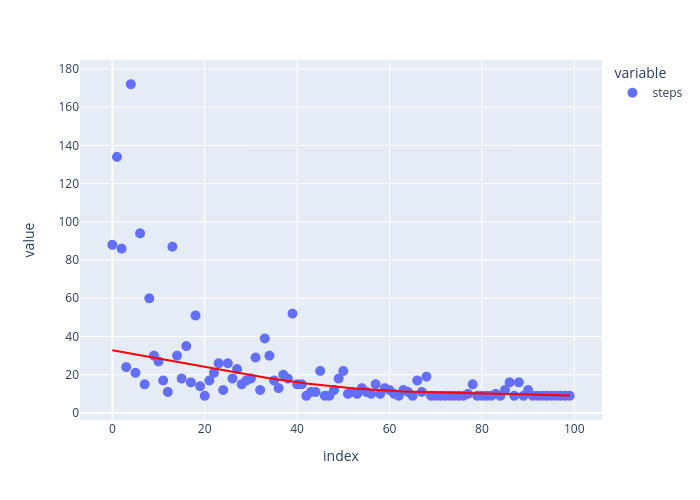
\includegraphics[width=.45\textwidth]{rl_into/windyworld_sarsa.png} & 
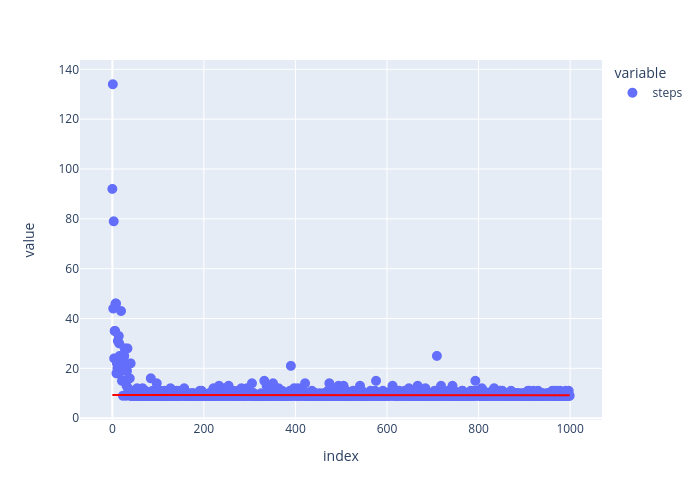
\includegraphics[width=.45\textwidth]{rl_into/windyworld_q_learning.png} 
\end{tabular}
\caption{SARSA and Q-Learning Results on Windyworld}
\label{fig:sarsaqlearning}
\end{figure}

\section{Review Questions}

\paragraph*{Introduction}
\begin{enumerate}[nosep]
\item What is reinforcement learning and how does it differ from other types of machine learning?
\item What is meant by the term ''model'' in the context of reinforcement learning?
\item Discuss the challenges associated with the stochastic nature of the environment in reinforcement learning.
\item Define the following terms and explain their significance in reinforcement learning:
\begin{itemize}
\item Policy ($\pi$)
\item Reward ($R$)
\item Return ($G$)
\item State value function ($v$)
\item Action value function ($q$)
\item Model ($p$)
\end{itemize}
\item Explain the difference between a deterministic policy and a stochastic policy. Provide an example of each from any real-world scenario.
\item Describe the general process of updating the value function. Include the update rule equation and explain each component.
\item Explain the significance of the action value function in the reinforcement learning framework. How does it differ from the state value function in terms of utility and information provided to the agent?
\item Discuss how reinforcement learning can be applied to customer interaction management and financial portfolio management. What are the potential benefits and challenges?
\item Consider the manufacturing process optimization application of reinforcement learning. Describe how an RL algorithm could continuously improve the process and what metrics it might focus on.
\item Discuss the implications of the exploration-exploitation trade-off in a non-gaming business scenario. How might a company balance these two aspects effectively?
\item Reflect on the potential impacts of reinforcement learning on customer satisfaction in a service-oriented business. What are the risks and rewards?
\item What role does the discount factor $\gamma$ play in calculating the return in a reinforcement learning problem? Why might one use a smaller or larger value of $\gamma$?
\end{enumerate}

\paragraph*{Questions on K-Armed Bandits}

\begin{enumerate}[nosep,resume*]
\item Why is the k-armed bandit problem considered to be a "stateless" problem in reinforcement learning?
\item Describe the action value function $Q_t(a)$ in the k-armed bandit problem. What does it represent?
\item Explain the concept of the $\epsilon$-greedy policy. How does it balance the exploration-exploitation trade-off?
\item Consider the incremental update formula used in the k-armed bandit problem and explain each term:
$Q_{t+1}(a) = Q_t(a) + \frac{1}{t} [R_t(a)-Q_t(a)]$. How does this formula ensure that the estimate becomes more accurate over time?
\item What are the implications of setting a higher or lower $\epsilon$ value in terms of long-term gains vs. short-term exploration?
\item Discuss the rationale behind using an "optimistic" initial value for the action-value estimates. How does this approach influence the agent's behavior?
\end{enumerate}

\paragraph*{Questions on Markov Decision Processes and Dynamic Programming}

\begin{enumerate}[nosep,resume*]
\item Define a Markov Decision Process (MDP) and explain the Markov property in this context.
\item Draw a figure of an RL agent and environment interaction; describe the roles of $S_t$, $A_t$, and $R_t$.
\item Explain what is meant by a \emph{trajectory} in the context of reinforcement learning.
\item Define the environment's dynamics using the \emph{p-function} and discuss its importance in MDPs.
\item Define the \emph{state value function} $v_\pi(s)$ and explain how it is used to evaluate a policy $\pi$.
\item Similarly, define the \emph{action value function} $q_\pi(s, a)$ and explain its relevance in policy evaluation.
\item Detail how the Bellman equation provides a recursive way to compute the value of a state under a specific policy.
\item Describe how iterative policy evaluation can be used to approximate the state value function before performing policy improvement.
\item Explain the process of \emph{iterative policy improvement} and how it leads to finding an optimal policy.
\end{enumerate}

\paragraph*{Questions on Monte Carlo (MC) Learning}

\begin{enumerate}[nosep,resume*]
\item Explain the fundamental concept of Monte Carlo (MC) learning in the context of reinforcement learning.
\item Define and distinguish between episodic tasks and continuous tasks in reinforcement learning.
\item Explain the difference between first-visit and every-visit MC methods. What are the implications of each approach on the learning process?
\item Describe the process of First-Visit Monte Carlo prediction as pseudocode. How does it update the state value function?
\item What is the purpose of the backward computation of the return $G$ in the first-visit MC prediction algorithm?
\item Explain the concept of ''exploring starts'' in the context of MC control and why it is necessary.
\item How do Monte Carlo methods handle the trade-off between exploration and exploitation, especially in environments where exploring starts are not feasible?
\item How does the game of Blackjack illustrate the application of Monte Carlo methods in episodic RL problems?
\item Analyze the potential impact of episodic task length on the effectiveness of Monte Carlo methods. What happens as the length of episodes increases?
\item How do Monte Carlo methods adapt when the environment's dynamics change over time?
\item Reflect on how Monte Carlo methods might perform in real-world scenarios such as financial markets or automated driving systems.
\end{enumerate}

\paragraph*{Questions on Off-Policy Monte Carlo (MC) Learning}

\begin{enumerate}[nosep,resume*]
\item Explain the difference between on-policy and off-policy learning methods in the context of Monte Carlo (MC) methods.
\item How does off-policy learning address the exploration-exploitation dilemma differently than on-policy learning?
\item Discuss why it is important for the behavior policy to cover the target policy in off-policy MC learning.
\item How does the update formula in off-policy MC control differ from the one used in on-policy MC control?
\item In the pseudocode for off-policy MC control, why is the episode terminated early if the action taken does not match the action recommended by the target policy?
\item Explain the potential impacts of the choice of behavior policy on the efficiency and effectiveness of off-policy learning.
\item Discuss how off-policy learning can be applied to complex environments where safety or cost constraints limit exploration.
\item Describe a scenario in which off-policy learning would be particularly advantageous over on-policy learning.
\item How can off-policy MC control be adapted to environments where the behavior policy cannot sufficiently cover the target policy?
\end{enumerate}

\paragraph*{Questions on Temporal-Difference (TD) Learning}

\begin{enumerate}[nosep,resume*]
\item What is temporal-difference (TD) learning and how does it differ from Monte Carlo methods?
\item Explain the concept of bootstrapping in the context of TD learning.
\item Discuss the advantages of TD learning in terms of update frequency and applicability to different types of environments.
\item Describe the SARSA algorithm and explain how it uses the TD update formula.
\item How can the SARSA algorithm be adjusted to improve its performance in highly dynamic environments?
\item Discuss how TD learning methods can be adapted to continuous (non-episodic) environments. What are the implications for learning in such environments?
\item Compare the convergence properties of TD learning and Monte Carlo methods. Why might TD learning converge faster in practical applications?
\item Explain the concept of "n-step TD learning." How does it extend the basic idea of TD learning?
\item What are the implications of using different "n" values in n-step TD learning on the performance and speed of learning?
\item Explain how n-step TD learning might provide a more stable learning update compared to one-step TD updates.
\item Provide an example scenario where TD learning might significantly outperform Monte Carlo methods in terms of learning efficiency and accuracy.
\end{enumerate}

\paragraph*{Questions on Off-Policy Temporal-Difference (TD) Learning}

\begin{enumerate}[nosep,resume*]
\item Describe the main difference between the update rules of SARSA and Q-learning. How does this difference define each as either on-policy or off-policy?
\item Explain how the Q-learning update rule ensures that the learning is directed towards the optimal policy.
\item What are the implications of using the $\operatorname*{max}_a Q(S', A')$ term in the Q-learning update rule? Discuss how this term influences the policy improvement process.
\item How does Q-learning handle the exploration-exploitation trade-off differently compared to SARSA?
\item How does the initial setting of Q-values influence the learning process and eventual performance in Q-learning? Discuss the impact of optimistic versus pessimistic initialization.
\end{enumerate}
